% Options for packages loaded elsewhere
\PassOptionsToPackage{unicode}{hyperref}
\PassOptionsToPackage{hyphens}{url}
%
\documentclass[
]{book}
\usepackage{amsmath,amssymb}
\usepackage{iftex}
\ifPDFTeX
  \usepackage[T1]{fontenc}
  \usepackage[utf8]{inputenc}
  \usepackage{textcomp} % provide euro and other symbols
\else % if luatex or xetex
  \usepackage{unicode-math} % this also loads fontspec
  \defaultfontfeatures{Scale=MatchLowercase}
  \defaultfontfeatures[\rmfamily]{Ligatures=TeX,Scale=1}
\fi
\usepackage{lmodern}
\ifPDFTeX\else
  % xetex/luatex font selection
\fi
% Use upquote if available, for straight quotes in verbatim environments
\IfFileExists{upquote.sty}{\usepackage{upquote}}{}
\IfFileExists{microtype.sty}{% use microtype if available
  \usepackage[]{microtype}
  \UseMicrotypeSet[protrusion]{basicmath} % disable protrusion for tt fonts
}{}
\makeatletter
\@ifundefined{KOMAClassName}{% if non-KOMA class
  \IfFileExists{parskip.sty}{%
    \usepackage{parskip}
  }{% else
    \setlength{\parindent}{0pt}
    \setlength{\parskip}{6pt plus 2pt minus 1pt}}
}{% if KOMA class
  \KOMAoptions{parskip=half}}
\makeatother
\usepackage{xcolor}
\usepackage{color}
\usepackage{fancyvrb}
\newcommand{\VerbBar}{|}
\newcommand{\VERB}{\Verb[commandchars=\\\{\}]}
\DefineVerbatimEnvironment{Highlighting}{Verbatim}{commandchars=\\\{\}}
% Add ',fontsize=\small' for more characters per line
\usepackage{framed}
\definecolor{shadecolor}{RGB}{248,248,248}
\newenvironment{Shaded}{\begin{snugshade}}{\end{snugshade}}
\newcommand{\AlertTok}[1]{\textcolor[rgb]{0.94,0.16,0.16}{#1}}
\newcommand{\AnnotationTok}[1]{\textcolor[rgb]{0.56,0.35,0.01}{\textbf{\textit{#1}}}}
\newcommand{\AttributeTok}[1]{\textcolor[rgb]{0.13,0.29,0.53}{#1}}
\newcommand{\BaseNTok}[1]{\textcolor[rgb]{0.00,0.00,0.81}{#1}}
\newcommand{\BuiltInTok}[1]{#1}
\newcommand{\CharTok}[1]{\textcolor[rgb]{0.31,0.60,0.02}{#1}}
\newcommand{\CommentTok}[1]{\textcolor[rgb]{0.56,0.35,0.01}{\textit{#1}}}
\newcommand{\CommentVarTok}[1]{\textcolor[rgb]{0.56,0.35,0.01}{\textbf{\textit{#1}}}}
\newcommand{\ConstantTok}[1]{\textcolor[rgb]{0.56,0.35,0.01}{#1}}
\newcommand{\ControlFlowTok}[1]{\textcolor[rgb]{0.13,0.29,0.53}{\textbf{#1}}}
\newcommand{\DataTypeTok}[1]{\textcolor[rgb]{0.13,0.29,0.53}{#1}}
\newcommand{\DecValTok}[1]{\textcolor[rgb]{0.00,0.00,0.81}{#1}}
\newcommand{\DocumentationTok}[1]{\textcolor[rgb]{0.56,0.35,0.01}{\textbf{\textit{#1}}}}
\newcommand{\ErrorTok}[1]{\textcolor[rgb]{0.64,0.00,0.00}{\textbf{#1}}}
\newcommand{\ExtensionTok}[1]{#1}
\newcommand{\FloatTok}[1]{\textcolor[rgb]{0.00,0.00,0.81}{#1}}
\newcommand{\FunctionTok}[1]{\textcolor[rgb]{0.13,0.29,0.53}{\textbf{#1}}}
\newcommand{\ImportTok}[1]{#1}
\newcommand{\InformationTok}[1]{\textcolor[rgb]{0.56,0.35,0.01}{\textbf{\textit{#1}}}}
\newcommand{\KeywordTok}[1]{\textcolor[rgb]{0.13,0.29,0.53}{\textbf{#1}}}
\newcommand{\NormalTok}[1]{#1}
\newcommand{\OperatorTok}[1]{\textcolor[rgb]{0.81,0.36,0.00}{\textbf{#1}}}
\newcommand{\OtherTok}[1]{\textcolor[rgb]{0.56,0.35,0.01}{#1}}
\newcommand{\PreprocessorTok}[1]{\textcolor[rgb]{0.56,0.35,0.01}{\textit{#1}}}
\newcommand{\RegionMarkerTok}[1]{#1}
\newcommand{\SpecialCharTok}[1]{\textcolor[rgb]{0.81,0.36,0.00}{\textbf{#1}}}
\newcommand{\SpecialStringTok}[1]{\textcolor[rgb]{0.31,0.60,0.02}{#1}}
\newcommand{\StringTok}[1]{\textcolor[rgb]{0.31,0.60,0.02}{#1}}
\newcommand{\VariableTok}[1]{\textcolor[rgb]{0.00,0.00,0.00}{#1}}
\newcommand{\VerbatimStringTok}[1]{\textcolor[rgb]{0.31,0.60,0.02}{#1}}
\newcommand{\WarningTok}[1]{\textcolor[rgb]{0.56,0.35,0.01}{\textbf{\textit{#1}}}}
\usepackage{longtable,booktabs,array}
\usepackage{calc} % for calculating minipage widths
% Correct order of tables after \paragraph or \subparagraph
\usepackage{etoolbox}
\makeatletter
\patchcmd\longtable{\par}{\if@noskipsec\mbox{}\fi\par}{}{}
\makeatother
% Allow footnotes in longtable head/foot
\IfFileExists{footnotehyper.sty}{\usepackage{footnotehyper}}{\usepackage{footnote}}
\makesavenoteenv{longtable}
\usepackage{graphicx}
\makeatletter
\def\maxwidth{\ifdim\Gin@nat@width>\linewidth\linewidth\else\Gin@nat@width\fi}
\def\maxheight{\ifdim\Gin@nat@height>\textheight\textheight\else\Gin@nat@height\fi}
\makeatother
% Scale images if necessary, so that they will not overflow the page
% margins by default, and it is still possible to overwrite the defaults
% using explicit options in \includegraphics[width, height, ...]{}
\setkeys{Gin}{width=\maxwidth,height=\maxheight,keepaspectratio}
% Set default figure placement to htbp
\makeatletter
\def\fps@figure{htbp}
\makeatother
\setlength{\emergencystretch}{3em} % prevent overfull lines
\providecommand{\tightlist}{%
  \setlength{\itemsep}{0pt}\setlength{\parskip}{0pt}}
\setcounter{secnumdepth}{5}
\usepackage{booktabs}
\usepackage{amsthm}
\usepackage{amsmath}
\usepackage[pagebackref=true,breaklinks=true,letterpaper=true,colorlinks,bookmarks=true]{hyperref}
\usepackage{tcolorbox}
\usepackage{color}
\usepackage{framed}
\setlength{\fboxsep}{.8em}
\makeatletter
\def\thm@space@setup{%
  \thm@preskip=8pt plus 2pt minus 4pt
  \thm@postskip=\thm@preskip
}
\makeatother

% \newcommand{\Real}[1]{\mathbb{R}^{#1}}
% \newcommand{\sym}[1]{\mathbb{S}^{#1}}
% \newcommand{\psd}[1]{\sym{#1}_{+}}
% \newcommand{\pd}[1]{\sym{#1}_{++}}
% \newcommand{\inprod}[2]{\langle #1, #2 \rangle}
% \newcommand{\linprod}[2]{\left\langle #1, #2 \right\rangle}
% \newcommand{\trace}{\mathrm{tr}}
% \newcommand{\tran}{^\top}
% % \newcommand{\det}{\mathrm{det}}
% \newcommand{\rank}{\mathrm{rank}}
% \newcommand{\diag}{\mathrm{diag}}

\newtcolorbox{examplebox}{
  colback=green,
  colframe=orange,
  coltext=black,
  boxsep=5pt,
  arc=4pt}

\newtcolorbox{theorembox}{
  colback=green,
  colframe=green,
  coltext=black,
  boxsep=5pt,
  arc=4pt}

\newtcolorbox{definitionbox}{
colback=white,
colframe=green,
coltext=black,
boxsep=5pt,
arc=4pt}
\ifLuaTeX
  \usepackage{selnolig}  % disable illegal ligatures
\fi
\usepackage[]{natbib}
\bibliographystyle{apalike}
\IfFileExists{bookmark.sty}{\usepackage{bookmark}}{\usepackage{hyperref}}
\IfFileExists{xurl.sty}{\usepackage{xurl}}{} % add URL line breaks if available
\urlstyle{same}
\hypersetup{
  pdftitle={Semidefinite Optimization and Relaxation},
  pdfauthor={Heng Yang},
  hidelinks,
  pdfcreator={LaTeX via pandoc}}

\title{Semidefinite Optimization and Relaxation}
\author{Heng Yang}
\date{2024-01-30}

\usepackage{amsthm}
\newtheorem{theorem}{Theorem}[chapter]
\newtheorem{lemma}{Lemma}[chapter]
\newtheorem{corollary}{Corollary}[chapter]
\newtheorem{proposition}{Proposition}[chapter]
\newtheorem{conjecture}{Conjecture}[chapter]
\theoremstyle{definition}
\newtheorem{definition}{Definition}[chapter]
\theoremstyle{definition}
\newtheorem{example}{Example}[chapter]
\theoremstyle{definition}
\newtheorem{exercise}{Exercise}[chapter]
\theoremstyle{definition}
\newtheorem{hypothesis}{Hypothesis}[chapter]
\theoremstyle{remark}
\newtheorem*{remark}{Remark}
\newtheorem*{solution}{Solution}
\begin{document}
\maketitle

{
\setcounter{tocdepth}{1}
\tableofcontents
}
\newcommand{\calQ}{\mathcal{Q}}
\newcommand{\calA}{\mathcal{A}}

\newcommand{\Real}[1]{\mathbb{R}^{#1}}
\newcommand{\sym}[1]{\mathbb{S}^{#1}}
\newcommand{\psd}[1]{\sym{#1}_{+}}
\newcommand{\pd}[1]{\sym{#1}_{++}}
\newcommand{\inprod}[2]{\langle #1, #2 \rangle}
\newcommand{\linprod}[2]{\left\langle #1, #2 \right\rangle}
\newcommand{\trace}{\mathrm{tr}}
\newcommand{\tran}{^\top}

\newcommand{\rank}{\mathrm{rank}}
\newcommand{\diag}{\mathrm{diag}}
\newcommand{\Diag}{\mathrm{Diag}}
\newcommand{\BlkDiag}{\mathrm{BlkDiag}}
\newcommand{\vectorize}{\mathrm{vec}}
\newcommand{\svec}{\mathrm{svec}}
\newcommand{\mat}{\mathrm{mat}}
\newcommand{\smat}{\mathrm{smat}}
\newcommand{\norm}[1]{\Vert #1 \Vert}
\newcommand{\lnorm}[1]{\left\Vert #1 \right\Vert}
\newcommand{\pnorm}[2]{\Vert #1 \Vert_{#2}}
\newcommand{\Fnorm}[1]{\Vert #1 \Vert_\mathrm{F}}
\newcommand{\conv}{\mathrm{conv}}
\newcommand{\cone}{\mathrm{cone}}
\newcommand{\interior}{\mathrm{int}}
\newcommand{\relint}{\mathrm{ri}}
\newcommand{\poly}[1]{\mathbb{R}[#1]}
\newcommand{\SOd}{\mathrm{SO}(d)}
\newcommand{\SOthree}{\mathrm{SO}(3)}
\newcommand{\Od}{\mathrm{O}(d)}
\newcommand{\Ogroup}{\mathrm{O}}
\newcommand{\usphere}{\mathcal{S}}
\newcommand{\bmath}[1]{\boldsymbol{#1}}
\newcommand{\lbrkt}{[\![}
\newcommand{\rbrkt}{]\!]}
\newcommand{\brkt}[1]{\lbrkt #1 \rbrkt}

\newcommand{\cbrace}[1]{\{ #1 \}}
\newcommand{\lcbrace}[1]{ \left\{ #1 \right\} }
\newcommand{\aff}{\mathrm{aff}}
\newcommand{\bbN}{\mathbb{N}}
\newcommand{\dist}{\mathrm{dist}}
\newcommand{\subject}{\mathrm{s.t.}}
\newcommand{\cl}{\mathrm{cl}}
\newcommand{\eye}{\mathrm{I}}
\newcommand{\inv}{^{-1}}
\newcommand{\Range}{\mathrm{Range}}
\renewcommand{\ker}{\mathrm{ker}}
\newcommand{\face}{\mathrm{face}}
\newcommand{\lmid}{\ \middle\vert\ }

\hypertarget{preface}{%
\chapter*{Preface}\label{preface}}
\addcontentsline{toc}{chapter}{Preface}

This is the textbook for Harvard ENG-SCI 257: Semidefinite Optimization and Relaxation.

\hypertarget{feedback}{%
\section*{Feedback}\label{feedback}}
\addcontentsline{toc}{section}{Feedback}

I would like to invite you to provide comments to the textbook via the following two ways:

\begin{itemize}
\tightlist
\item
  Inline comments with Hypothesis:

  \begin{itemize}
  \tightlist
  \item
    Go to \href{https://hypothes.is}{Hypothesis} and create an account
  \item
    Install the \href{https://chrome.google.com/webstore/detail/hypothesis-web-pdf-annota/bjfhmglciegochdpefhhlphglcehbmek}{Chrome extension of Hypothesis}
  \item
    Provide public comments to textbook contents and I will try to address them
  \end{itemize}
\item
  Blog-style comments with Disqus:

  \begin{itemize}
  \tightlist
  \item
    At the end of each Chapter, there is a Disqus module where you can leave feedback
  \end{itemize}
\end{itemize}

I would recommend using Disqus for high-level and general feedback regarding the entire Chapter, but using Hypothesis for feedback and questions about the technical details.

\hypertarget{offerings}{%
\section*{Offerings}\label{offerings}}
\addcontentsline{toc}{section}{Offerings}

Information about the offerings of the class is listed below.

\hypertarget{spring}{%
\subsubsection*{2024 Spring}\label{spring}}
\addcontentsline{toc}{subsubsection}{2024 Spring}

\textbf{Time}: Mon/Wed 2:15 - 3:30pm

\textbf{Location}: Science and Engineering Complex, 1.413

\textbf{Instructor}: \href{https://hankyang.seas.harvard.edu/}{Heng Yang}

\textbf{Teaching Fellow}: \href{https://safwanhossain.github.io/}{Safwan Hossain}

\href{https://docs.google.com/document/d/1H6Wqht_PVw_n8Jl0kXN3HjZfHkeZJYqYWT4ayxvqRlU/edit?usp=sharing}{\textbf{Syllabus}}

\hypertarget{notation}{%
\chapter*{Notation}\label{notation}}
\addcontentsline{toc}{chapter}{Notation}

We will use the following standard notation throughout this book.

\textbf{Basics}

\begin{longtable}[]{@{}
  >{\raggedright\arraybackslash}p{(\columnwidth - 2\tabcolsep) * \real{0.7083}}
  >{\raggedright\arraybackslash}p{(\columnwidth - 2\tabcolsep) * \real{0.2917}}@{}}
\toprule\noalign{}
\endhead
\bottomrule\noalign{}
\endlastfoot
\(\mathbb{R}^{}\) & real numbers \\
\(\mathbb{R}^{}_{+}\) & nonnegative real \\
\(\mathbb{R}^{}_{++}\) & positive real \\
\(\mathbb{Z}\) & integers \\
\(\mathbb{N}\) & nonnegative integers \\
\(\mathbb{N}_{+}\) & positive integers \\
\(\mathbb{R}^{n}\) & \(n\)-D column vector \\
\(\mathbb{R}^{n}_{+}\) & nonnegative orthant \\
\(\mathbb{R}^{n}_{++}\) & positive orthant \\
\(e_i\) & standard basic vector \\
\(\Delta_n := \{x \in \mathbb{R}^n_{+} \mid \sum x_i = 1 \}\) & standard simplex \\
\end{longtable}

\textbf{Matrices}

\begin{longtable}[]{@{}
  >{\raggedright\arraybackslash}p{(\columnwidth - 2\tabcolsep) * \real{0.7083}}
  >{\raggedright\arraybackslash}p{(\columnwidth - 2\tabcolsep) * \real{0.2917}}@{}}
\toprule\noalign{}
\endhead
\bottomrule\noalign{}
\endlastfoot
\(\mathbb{R}^{m \times n}\) & \(m \times n\) real matrices \\
\(\mathbb{S}^{n}\) & \(n\times n\) symmetric matrices \\
\(\mathbb{S}^{n}_{+}\) & \(n\times n\) positive semidefinite matrices \\
\(\mathbb{S}^{n}_{++}\) & \(n\times n\) positive definite matrices \\
\(\langle A, B \rangle\) or \(\bullet\) & inner product in \(\mathbb{R}^{m \times n}\) \\
\(\mathrm{tr}(A)\) & trace of \(A \in \mathbb{R}^{n \times n}\) \\
\(A^\top\) & matrix transpose \\
\(\det(A)\) & matrix determinant \\
\(\mathrm{rank}(A)\) & rank of a matrix \\
\(\mathrm{diag}(A)\) & diagonal of a matrix \(A\) as a vector \\
\(\mathrm{Diag}(a)\) & turning a vector into a diagonal matrix \\
\(\mathrm{BlkDiag}(A,B,\dots)\) & block diagonal matrix with blocks \(A,B,\dots\) \\
\(\succeq 0\) and \(\preceq 0\) & positive / negative semidefinite \\
\(\succ 0\) and \(\prec 0\) & positive / negative definite \\
\(\lambda_{\max}\) and \(\lambda_{\min}\) & maximum / minimum eigenvalue \\
\(\sigma_{\max}\) and \(\sigma_{\min}\) & maximum / minimum singular value \\
\(\mathrm{vec}(A)\) & vectorization of \(A \in \mathbb{R}^{m \times n}\) \\
\(\mathrm{svec}(A)\) & symmetric vectorization of \(A \in \mathbb{S}^{n}\) \\
\(\Vert A \Vert_\mathrm{F}\) & Frobenius norm \\
\(\mathrm{Range}(A)\) & span of the column vectors \\
\(\mathrm{ker}(A)\) & right null space \\
\end{longtable}

\textbf{Geometry}

\begin{longtable}[]{@{}ll@{}}
\toprule\noalign{}
\endhead
\bottomrule\noalign{}
\endlastfoot
\(\Vert a \Vert_{p}\) & \(p\)-norm \\
\(\Vert a \Vert\) & \(2\)-norm \\
\(B(o,r)\) & ball with center \(o\) and radius \(r\) \\
\(\mathrm{aff}(S)\) & affine hull of set \(S\) \\
\(\mathrm{conv}(S)\) & convex hull of set \(S\) \\
\(\mathrm{cone}(S)\) & conical hull of set \(S\) \\
\(\mathrm{int}(S)\) & interior of set \(S\) \\
\(\mathrm{ri}(S)\) & relative interior of set \(S\) \\
\(\partial S\) & boundary of set \(S\) \\
\(P^\circ\) & polar of convex body \\
\(P^{*}\) & dual of set \(P\) \\
\(\mathrm{O}(d)\) & orthogonal group of dimension \(d\) \\
\(\mathrm{SO}(d)\) & special orthogonal group of dimension \(d\) \\
\(\mathcal{S}^{d-1}\) & unit sphere in \(\mathbb{R}^{d}\) \\
\end{longtable}

\textbf{Optimization}

\begin{longtable}[]{@{}ll@{}}
\toprule\noalign{}
\endhead
\bottomrule\noalign{}
\endlastfoot
KKT & Karush--Kuhn--Tucker \\
LP & linear program \\
QP & quadratic program \\
SOCP & second-order cone program \\
SDP & semidefinite program \\
\end{longtable}

\textbf{Algebra}

\begin{longtable}[]{@{}ll@{}}
\toprule\noalign{}
\endhead
\bottomrule\noalign{}
\endlastfoot
\(\mathbb{R}[x]\) & polynomial ring in \(x\) with real coefficients \\
\(\deg\) & degree of a monomial / polynomial \\
\(\mathbb{R}[x]_d\) & polynomials in \(x\) of degree up to \(d\) \\
\([x]_d\) & vector of monomials of degree up to \(d\) \\
\([\![x ]\!]_d\) & vector of monomials of degree \(d\) \\
\end{longtable}

\hypertarget{background}{%
\chapter{Mathematical Background}\label{background}}

\hypertarget{background:convexity}{%
\section{Convexity}\label{background:convexity}}

A very important notion in modern optimization is that of \emph{convexity}. To a large extent, an optimization problem is ``easy'' if it is convex, and ``difficult'' when convexity is lost, i.e., \emph{nonconvex}. We give a basic review of convexity here and refer the reader to \citep{rockafellar70-convexanalysis}, \citep{boyd04book-convex}, and \citep{bertsekas03book-convex} for comprehensive treatments.

We will work on a finite-dimensional real vector space, which we will identify with \(\mathbb{R}^{n}\).

\begin{definition}[Convex Set]
\protect\hypertarget{def:ConvexSet}{}\label{def:ConvexSet}A set \(S\) is convex if \(x_1,x_2 \in S\) implies \(\lambda x_1 + (1-\lambda) x_2 \in S\) for any \(\lambda \in [0,1]\). In other words, if \(x_1,x_2 \in S\), then the line segment connecting \(x_1\) and \(x_2\) lies inside \(S\).
\end{definition}

Conversely, a set \(S\) is nonconvex if Definition \ref{def:ConvexSet} does not hold.

Given \(x_1, x_2 \in S\), \(\lambda x_1 + (1-\lambda) x_2\) is called a \emph{convex combination} when \(\lambda \in [0,1]\). For convenience, we will use the following notation
\begin{equation}
\begin{split}
(x_1,x_2) = \{ \lambda x_1 + (1-\lambda) x_2 \mid \lambda \in (0,1) \}, \\ [x_1,x_2] = \{ \lambda x_1 + (1-\lambda) x_2 \mid \lambda \in [0,1] \}.
\end{split}
\end{equation}

A \textbf{hyperplane} is a common convex set defined as
\begin{equation}
H = \{  x \in \mathbb{R}^{n} \mid \langle c, x \rangle = d  \}
\label{eq:hyperplane}
\end{equation}
for some \(c \in \mathbb{R}^{n}\) and scalar \(d\). A \textbf{halfspace} is a convex set defined as
\begin{equation}
H^{+} = \{  x \in \mathbb{R}^{n} \mid \langle c, x \rangle \geq d  \}.
\label{eq:halfspace}
\end{equation}

Given two nonempty convex sets \(C_1\) and \(C_2\), the \textbf{distance} between \(C_1\) and \(C_2\) is defined as
\begin{equation}
\mathrm{dist}(C_1,C_2) = \inf \{ \Vert c_1 - c_2 \Vert \mid c_1 \in C_1, c_2 \in C_2 \}.
\end{equation}

For a convex set \(C\), the hyperplane \(H\) in \eqref{eq:hyperplane} is called a \textbf{supporting hyperplane} for \(C\) if \(C\) is contained in the half space \(H^{+}\) and the distance between \(H\) and \(C\) is zero. For example, the hyperplane \(x_1 = 0\) is supporting for the hyperboloid \(\{ (x_1,x_2) \mid x_1 x_2 \geq 1, x_1 \geq 0, x_2 \geq 0 \}\) in \(\mathbb{R}^{2}\).

An important property of a convex set is that we can \emph{certify} when a point is not in the set. This is usually done via a separation theorem.

\begin{theorem}[Separation Theorem]
\protect\hypertarget{thm:SeparationTheorem}{}\label{thm:SeparationTheorem}Let \(S_1,S_2\) be two convex sets in \(\mathbb{R}^{n}\) and \(S_1 \cap S_2 = \emptyset\), then there exists a hyperplane that separates \(S_1\) and \(S_2\), i.e., there exists \(c\) and \(d\) such that
\begin{equation}
\begin{split}
\langle c, x \rangle \geq d, &  \forall x \in S_1,\\
\langle c, x \rangle \leq d, & \forall x \in S_2.
\end{split}
\label{eq:separation}
\end{equation}
Further, if \(S_1\) is compact (i.e., closed and bounded) and \(S_2\) is closed, then the separation is strict, i.e., the inequalities in \eqref{eq:separation} are strict.
\end{theorem}

The strict separation theorem is used typically when \(S_1\) is a single point (hence compact).

We will see a generalization of the separation theorem for nonconvex sets later after we introduce the idea of sums of squares.

\begin{exercise}
Provide examples of two disjoint convex sets such that the separation in \eqref{eq:separation} is not strict in one way and both ways.
\end{exercise}

\begin{exercise}
Provide a constructive proof that the separation hyperplane exists in Theorem \ref{thm:SeparationTheorem} when (1) both \(S_1\) and \(S_2\) are closed, and (2) at least one of them is bounded.
\end{exercise}

The intersection of convex sets is always convex (try to prove this).

\hypertarget{background:convex:geometry}{%
\section{Convex Geometry}\label{background:convex:geometry}}

\hypertarget{basic-facts}{%
\subsection{Basic Facts}\label{basic-facts}}

Given a set \(S\), its \textbf{affine hull} is the set
\[
\mathrm{aff}(S) =  \left\{  \sum_{i=1}^k \lambda_i u_i \mid \lambda_1 + \dots + \lambda_k = 1, u_i \in S, k \in \mathbb{N}_{+}  \right\} ,
\]
where \(\sum_{i=1}^{k} \lambda_i u_i\) is called an \emph{affine combination} of \(u_1,\dots,u_k\) when \(\sum_i \lambda_i = 1\). The affine hull of a set is the smallest affine subspace that contains \(S\), and the \textbf{dimension} of \(S\) is the dimension of its affine hull. The affine hull of the emptyset is the emptyset, of a singleton is the singleton itself. The affine hull of a set of two different points is the line going through them. The affine hull of a set of three points not on one line is the plane going through them. The affine hull of a set of four points not in a plane in \(\mathbb{R}^{3}\) is the entire space \(\mathbb{R}^{3}\).

For a convex set \(C \subseteq \mathbb{R}^{n}\), the \textbf{interior} of \(C\) is defined as
\[
\mathrm{int}(C) := \{  u \in C \mid \exists \epsilon > 0, B(u,\epsilon) \subseteq C  \},
\]
where \(B(u,\epsilon)\) denotes a ball centered at \(u\) with radius \(\epsilon\) (using the usual 2-norm). Each point in \(\mathrm{int}(C)\) is called an \emph{interior point} of \(C\). If \(\mathrm{int}(C) = C\), then \(C\) is said to be an \textbf{open set}. A convex set with nonempty interior is called a \textbf{convex domain}, while a compact (i.e., closed and bounded) convex domain is called a \textbf{convex body}.

The \textbf{boundary of \(C\)} is the subset of points that are in the \textbf{closure}\footnote{The closure of a subset \(C\) of points, denoted \(\mathrm{cl}(C)\), consists of all points in \(C\) together with all limit points of \(C\). The closure of \(C\) may equivalently be defined as the intersection of all closed sets containing \(C\). Intuitively, the closure can be thought of as all the points that are either in \(C\) or ``very near'' \(C\). For example, the closure of the open line segment \(C= (0,1)\) is the closed line segment \(C=[0,1]\).} of \(C\) but are not in the interior of \(C\), and we denote it as \(\partial C\). For example, the closed line segment \(C = [0,1]\) has two points on the boundary: \(0\) and \(1\); the open line segment \(C = (0,1)\) has the same two points as its boundary.

It is possible that a convex set has empty interior. For example, a hyperplane has no interior, and neither does a singleton. In such cases, the \textbf{relative interior} can be defined as
\[
\mathrm{ri}(C) := \{  u \in C \mid \exists \epsilon > 0, B(u,\epsilon) \cap \mathrm{aff}(C) \subseteq C  \}.
\]
For a nonempty convex set, the relative interior always exists. If \(\mathrm{ri}(C) = C\), then \(C\) is said to be \textbf{relatively open}. For example, the relative interior of a singleton is the singleton itself, and hence a singleton is relatively open.

For a convex set \(C\), a point \(u \in C\) is called an \textbf{extreme point} if
\[
u \in (x,y), x \in C, y \in C \quad \Rightarrow u = x = y.
\]
For example, consider \(C = \{ (x,y)\mid x^2 + y^2 \leq 1 \}\), then all the points on the boundary \(\partial C = \{ (x,y) \mid x^2 + y^2 = 1 \}\) are extreme points.

A subset \(F \subseteq C\) is called a \textbf{face} if \(F\) itself is convex and
\[
u \in (x,y), u \in F, x,y \in C \quad \Rightarrow x,y \in F. 
\]
Clearly, the empty set \(\emptyset\) and the entire set \(C\) are faces of \(C\), which are called \emph{trivial faces}. The face \(F\) is said to be \emph{proper} if \(F \neq C\). The set of any single extreme point is also a face. A face \(F\) of \(C\) is called \textbf{exposed} if there exists a supporting hyperplane \(H\) for \(C\) such that
\[
F = H \cap C.
\]

\hypertarget{cones-duality-polarity}{%
\subsection{Cones, Duality, Polarity}\label{cones-duality-polarity}}

\begin{definition}[Polar]
\protect\hypertarget{def:polar}{}\label{def:polar}For a nonempty set \(T \subseteq \mathbb{R}^{n}\), its polar is the set
\begin{equation}
T^\circ := \{  y \in \mathbb{R}^{n} \mid \langle x, y \rangle \leq 1, \forall x \in T  \}.
\label{eq:polar}
\end{equation}
\end{definition}

The polar \(T^\circ\) is a closed convex set and contains the origin. Note that \(T\) is always contained in the polar of \(T^\circ\), i.e., \(T \subseteq (T^\circ)^\circ\). Indeed, they are equal under some assumptions.

\begin{theorem}[Bipolar]
\protect\hypertarget{thm:bipolar}{}\label{thm:bipolar}If \(T \subseteq \mathbb{R}^{n}\) is a closed convex set containing the origin, then \((T^\circ)^\circ = T\).
\end{theorem}

An important class of convex sets are those that are invariant under positive scalings.\footnote{Some authors define a cone using nonnegative scalings.} A set \(K \subseteq \mathbb{R}^{n}\) is a \textbf{cone} if \(t x \in K\) for all \(x \in K\) and for all \(t > 0\). For example, the positive real line \(\{ x \in \mathbb{R}^{} \mid x > 0 \}\) is a cone. The cone \(K\) is \textbf{pointed} if \(K \cap -K = \{ 0 \}\). It is said to be \textbf{solid} if its interior \(\mathrm{int}(K) \neq \emptyset\). Any nonzero point of a cone cannot be extreme. If a cone is pointed, the only extreme point is the origin.

The analogue of extreme point for convex cones is the \textbf{extreme ray}. For a convex cone \(K\) and \(0 \neq u \in K\), the line segment
\[
u \cdot [0,\infty) := \{ tu \mid t\geq 0 \}
\]
is called an extreme ray of \(K\) if
\[
u \in (x,y), x,y \in K \quad \Rightarrow \quad u,x,y \text{ are parallel to each other}.
\]
If \(u \cdot [0,\infty)\) is an extreme ray, then we say \(u\) generates the extreme ray.

\begin{definition}[Proper Cone]
\protect\hypertarget{def:ProperCone}{}\label{def:ProperCone}A cone \(K\) is proper if it is closed, convex, pointed, and solid.
\end{definition}

A proper cone \(K\) induces a \textbf{partial order} on the vector space, via \(x \succeq y\) if \(x - y \in K\). We also use \(x \succ y\) if \(x - y\) is in \(\mathrm{int}(K)\). Important examples of proper cones are the nonnegative orthant, the second-order cone, the set of symmetric positive semidefinite matrices, and the set of nonnegative polynomials, which we will describe later in the book.

\begin{definition}[Dual]
\protect\hypertarget{def:Dual}{}\label{def:Dual}The dual of a nonempty set \(S\) is
\[
S^* := \{  y \in \mathbb{R}^{n} \mid \langle y, x \rangle \geq 0, \forall x \in S \}.
\]
\end{definition}

Given any set \(S\), its dual \(S^*\) is always a closed convex cone. Duality reverses inclusion, that is,
\[
S_1 \subseteq S_2 \quad \Rightarrow \quad S_1^* \supseteq S_2^*.
\]
If \(S\) is a closed convex cone, then \(S^{* *}= S\). Otherwise, \(S^{* *}\) is the closure of the smallest convex cone that contains \(S\).

For a cone \(K \subseteq \mathbb{R}^{n}\), one can show that
\[
K^\circ = \{ y \in \mathbb{R}^{n} \mid \langle x, y \rangle \leq 0, \forall x \in K \}.
\]
The set \(K^\circ\) is called the \textbf{polar cone} of \(K\). The negative of \(K^\circ\) is just the \textbf{dual cone}
\[
K^{*} = \{ y \in \mathbb{R}^{n} \mid \langle x, y \rangle \geq 0, \forall x \in K \}.
\]

\begin{definition}[Self-dual]
\protect\hypertarget{def:selfdual}{}\label{def:selfdual}A cone \(K\) is self-dual if \(K^{*} = K\).
\end{definition}

As an easy example, the nonnegative orthant \(\mathbb{R}^{n}_{+}\) is self-dual.

\begin{example}[Second-order Cone]
\protect\hypertarget{exm:SecondOrderCone}{}\label{exm:SecondOrderCone}The second-order cone, or the Lorentz cone, or the ice cream cone
\[
\mathcal{Q}_n := \{  (x_0,x_1,\dots,x_n) \in \mathbb{R}^{n+1} \mid \sqrt{x_1^2 + \dots + x_n^2} \leq x_0  \}
\]
is a proper cone of \(\mathbb{R}^{n+1}\). We will show that it is also self-dual.

\textbf{Proof}. Consider \((y_0,y_1,\dots,y_n) \in \mathcal{Q}_n\), we want to show that
\begin{equation}
x_0 y_0 + x_1 y_1 + \dots + x_n y_n \geq 0, \forall (x_0,x_1,\dots,x_n) \in \mathcal{Q}_n.
\label{eq:dual-cone-condition}
\end{equation}
This is easy to verify because
\[
x_1 y_1 + \dots + x_n y_n \geq - \sqrt{x_1^2 + \dots + x_n^2} \sqrt{y_1^2 + \dots + y_n^2} \geq - x_0 y_0.
\]
Hence we have \(\mathcal{Q}_n \subseteq \mathcal{Q}_n^{*}\).

Conversely, if \eqref{eq:dual-cone-condition} holds, then take
\[
x_1 = -y_1, \dots, x_n = - y_n, \quad x_0 = \sqrt{x_1^2 + \dots + x_n^2},
\]
we have
\[
y_0 \geq \sqrt{y_1^2 + \dots + y_n^2},
\]
hence \(\mathcal{Q}_n^{*} \subseteq \mathcal{Q}_n\). \(\blacksquare\)
\end{example}

Not every proper cone is self-dual.

\begin{exercise}
Consider the following proper cone in \(\mathbb{R}^{2}\)
\[
K = \{ (x_1,x_2) \mid 2x_1 - x_2 \geq 0, 2x_2 - x_1 \geq 0 \}.
\]
Show that it is not self-dual.
\end{exercise}

\hypertarget{background:convex:optimization}{%
\section{Convex Optimization}\label{background:convex:optimization}}

\begin{definition}[Convex Function]
\protect\hypertarget{def:ConvexFun}{}\label{def:ConvexFun}A function \(f: \mathbb{R}^{n} \rightarrow \mathbb{R}^{}\) is a convex function if
\[
f(\lambda x + (1-\lambda) y) \leq \lambda f(x) + (1-\lambda) f(y), \forall \lambda \in [0,1], \forall x,y \in \mathbb{R}^{n}.
\]
\end{definition}

A function \(f\) is convex if and only if its \textbf{epigraph} \(\{ (x,t) \in \mathbb{R}^{n+1} \mid f(x) \leq t \}\) is a convex set.

When a function \(f\) is differentiable, then there are several equivalent characterizations of convexity, in terms of the gradient \(\nabla f(x)\) or the Hessian \(\nabla^2 f(x)\).

\begin{theorem}[Equivalent Characterizations of Convexity]
\protect\hypertarget{thm:CharacterizeConvexity}{}\label{thm:CharacterizeConvexity}

Let \(f: \mathbb{R}^{n} \rightarrow \mathbb{R}^{}\) be a twice differentiable function. The following propositions are equivalent.

\begin{enumerate}
\def\labelenumi{\roman{enumi}.}
\item
  \(f\) is convex, i.e.,
  \[
  f(\lambda x + (1-\lambda) y) \leq \lambda f(x) + (1-\lambda) f(y), \forall \lambda \in [0,1], x,y \in \mathbb{R}^{n}.
  \]
\item
  The first-order convexity condition holds:
  \[
  f(y) \geq f(x) + \langle \nabla f(x),  y - x \rangle, \forall x, y \in \mathbb{R}^{n},
  \]
  i.e., the hyperplane going through \((x,f(x))\) with slope \(\nabla f(x)\) supports the epigraph of \(f\).
\item
  The second-order convexity condition holds:
  \[
  \nabla^2 f(x) \succeq 0, \forall x \in \mathbb{R}^{n},
  \]
  i.e., the Hessian is positive semidefinite everywhere.
\end{enumerate}

\end{theorem}

Let's work on a little exercise.

\begin{exercise}

Which one of the following functions \(f: \mathbb{R}^{n} \rightarrow \mathbb{R}^{}\) is not convex?

\begin{enumerate}
\def\labelenumi{\alph{enumi}.}
\item
  \(\exp(-c^\top x)\), with \(c\) constant
\item
  \(\exp(c^\top x)\), with \(c\) constant
\item
  \(\exp(x^\top x)\)
\item
  \(\exp(-x^\top x)\)
\end{enumerate}

\end{exercise}

\hypertarget{minimax-theorem}{%
\subsection{Minimax Theorem}\label{minimax-theorem}}

Given a function \(f: X \times Y \rightarrow \mathbb{R}^{}\), the following inequality always holds
\begin{equation}
\max_{y \in Y} \min_{x \in X} f(x,y) \leq \min_{x \in X} \max_{y \in Y} f(x,y).
\label{eq:weak-minimax}
\end{equation}
If the maximum or minimum is not attained, then \eqref{eq:weak-minimax} holds with \(\max\) / \(\min\) replaced by \(\sup\) and \(\inf\), respectively.

\begin{exercise}
Provide examples of \(f\) such that the inequality in \eqref{eq:weak-minimax} is strict.
\end{exercise}

It is of interest to understand when equality holds in \eqref{eq:weak-minimax}.

\begin{theorem}[Minimax Theorem]
\protect\hypertarget{thm:minimax}{}\label{thm:minimax}Let \(X \subset \mathbb{R}^{n}\) and \(Y \subset \mathbb{R}^{n}\) be compact convex sets, and \(f: X \times Y \rightarrow \mathbb{R}^{}\) be a continuous function that is convex in its first argument and concave in the second. Then
\[
\max_{y \in Y} \min_{x \in X} f(x,y) = \min_{x \in X} \max_{y \in Y} f(x,y).
\]
\end{theorem}

A special case of this theorem, used in game theory to prove the existence of equilibria for zero-sum games, is when \(X\) and \(Y\) are standard unit simplicies and the function \(f(x,y)\) is bilinear. In a research from our group \citep{tang23arxiv-uncertainty}, we used the minimax theorem to convert a minimax problem into a single-level minimization problem.

\hypertarget{background:convex:optimization:Lagrangian}{%
\subsection{Lagrangian Duality}\label{background:convex:optimization:Lagrangian}}

Consider a nonlinear optimization problem
\begin{equation}
\begin{split}
u^\star = \min_{x \in \mathbb{R}^{n}} & \quad f(x) \\
\mathrm{s.t.}& \quad g_i(x) \leq 0, i=1,\dots,m, \\
& \quad h_j(x) = 0, j = 1,\dots,p.
\end{split}
\label{eq:background-nlp}
\end{equation}
Define the \textbf{Lagrangian} associated with the optimization problem \eqref{eq:background-nlp} as
\begin{equation}
\begin{split}
L: \mathbb{R}^{n} \times \mathbb{R}^{m}_{+} \times \mathbb{R}^{p} \quad & \rightarrow \quad \mathbb{R}^{}, \\
(x,\lambda,\mu) \quad & \mapsto \quad f(x) + \sum_{i=1}^m \lambda_i g_i(x) + \sum_{j=1}^p \mu_j h_j(x).
\end{split}
\label{eq:background-Lagrangian}
\end{equation}
The \textbf{Lagrangian dual function} is defined as
\begin{equation}
\phi(\lambda,\mu) := \min_{x \in \mathbb{R}^{n}} L(x,\lambda,\mu).
\label{eq:background-Lagrangian-dual}
\end{equation}
Maximizing this function over the dual variables \((\lambda,\mu)\) yields
\begin{equation}
v^\star := \max_{\lambda \geq 0, \mu \in \mathbb{R}^{p}} \phi(\lambda,\mu)
\label{eq:background-Lagrangian-dual-problem}
\end{equation}
Applying the minimax Theorem \ref{thm:minimax}, we can see that
\[
v^\star = \max_{(\lambda,\mu)} \min_{x} L(x,\lambda,\mu) \leq \min_{x} \max_{(\lambda,\mu)} L(x,\lambda,\mu) = u^\star.
\]
That is to say solving the dual problem \eqref{eq:background-Lagrangian-dual-problem} always provides a lower bound to the primal problem \eqref{eq:background-nlp}.

If the functions \(f,g_i\) are convex and \(h_i\) are affine, the Lagrangian is convex in \(x\) and convex in \((\lambda,\mu)\). To ensure strong duality (i.e., \(u^\star = v^\star\)), compactness or other \textbf{constraint qualifications} are needed. An often used condition is the Slater constraint qualification.

\begin{definition}[Slater Constraint Qualification]
\protect\hypertarget{def:SlaterCQ}{}\label{def:SlaterCQ}There exists a strictly feasible point for \eqref{eq:background-nlp}, i.e., a point \(z \in \mathbb{R}^{n}\) such that \(h_j(z) = 0,j=1,\dots,p\) and \(g_i(z) < 0,i=1,\dots,m\).
\end{definition}

Under these conditions, we have strong duality.

\begin{theorem}[Strong Duality]
\protect\hypertarget{thm:StrongDuality}{}\label{thm:StrongDuality}Consider the optimization \eqref{eq:background-nlp} and assume \(f,g_i\) are convex and \(h_j\) are affine. If Slater's constraint qualification holds, then the optimal value of the primal problem \eqref{eq:background-nlp} is the same as the optimal value of the dual problem \eqref{eq:background-Lagrangian-dual-problem}.
\end{theorem}

\hypertarget{kkt-optimality-conditions}{%
\subsection{KKT Optimality Conditions}\label{kkt-optimality-conditions}}

Consider the nonlinear optimization problem \eqref{eq:background-nlp}. A pair of primal and dual variables \((x^\star,\lambda^\star,\mu^\star)\) is said to satisfy the Karush-Kuhn-Tucker (KKT) optimality conditions if

\begin{equation}
\begin{split}
\text{primal feasibility}:\ \  & g_i(x^\star) \leq 0,\forall i=1,\dots,m; h_j(x^\star) = 0, \forall j=1,\dots,p \\
\text{dual feasibility}:\ \  & \lambda_i^\star \geq 0, \forall i=1,\dots,m \\
\text{stationarity}:\ \  & \nabla_x L(x^\star,\lambda^\star,\mu^\star) = 0 \\
\text{complementarity}:\ \  & \lambda_i^\star \cdot g_i(x^\star) = 0, \forall i=1,\dots,m.
\end{split}
\label{eq:KKT-conditions}
\end{equation}

Under certain constraint qualifications, the KKT conditions are necessary for local optimality.

\begin{theorem}[Necessary Optimality Conditions]
\protect\hypertarget{thm:KKTNecessary}{}\label{thm:KKTNecessary}Assume any of the following constraint qualifications hold:

\begin{itemize}
\item
  The gradients of the constraints \(\{ \nabla g_i(x^\star) \}_{i=1}^m\), \(\{ \nabla h_j(x^\star) \}_{j=1}^p\) are linearly independent.
\item
  Slater's constraint qualification (cf.~Definition \ref{def:SlaterCQ}).
\item
  All constraints \(g_i(x)\) and \(h_j(x)\) are affine functions.
\end{itemize}

Then, at every local minimum \(x^\star\) of \eqref{eq:background-nlp}, the KKT conditions \eqref{eq:KKT-conditions} hold.
\end{theorem}

On the other hand, for convex optimization problems, the KKT conditions are sufficient for global optimality.

\begin{theorem}[Sufficient Optimality Conditions]
\protect\hypertarget{thm:KKTSufficient}{}\label{thm:KKTSufficient}Assume optimization \eqref{eq:background-nlp} is convex, i.e., \(f,g_i\) are convex and \(h_j\) are affine. Every point \(x^\star\) that satisfies the KKT conditions \eqref{eq:KKT-conditions} is a global minimizer.
\end{theorem}

\hypertarget{background:linear:optimization}{%
\section{Linear Optimization}\label{background:linear:optimization}}

\hypertarget{polyhedra}{%
\subsection{Polyhedra}\label{polyhedra}}

In \(\mathbb{R}^{n}\), a \textbf{polyhedron} is a set defined by finitely many linear inequalities, i.e.,
\begin{equation}
P = \{ x \in \mathbb{R}^{n} \mid A x \geq b \},
\label{eq:polyhedron}
\end{equation}
for some matrix \(A \in \mathbb{R}^{m \times n}\) and \(b \in \mathbb{R}^{m}\). In \eqref{eq:polyhedron}, the inequality should be interpreted as \(A x - b \in \mathbb{R}^{m}_{+}\), i.e., every entry of \(Ax\) is no smaller than the corresponding entry of \(b\).

The convex hull of finitely many points in \(\mathbb{R}^{n}\) is called a \textbf{polytope}, where the convex hull of a set \(S\) is defined as
\begin{equation}
\hspace{-10mm} \mathrm{conv}(S) =  \left\{ \sum_{i=1}^k \lambda_i u_i \mid k \in \mathbb{N}_{+}, \sum_{i=1}^k \lambda_i = 1, \lambda_i \geq 0,i=1,\dots,k, u_i \in S, \forall i =1,\dots,k \right\} ,
\label{eq:convex-hull}
\end{equation}
i.e., all possible convex combinations of points in \(S\). Clearly, a polytope is bounded.

The conic hull of finitely many points in \(\mathbb{R}^{n}\) is called a \textbf{polyhedral cone}, where the conic hull of a set \(S\) is defined as
\begin{equation}
\hspace{-10mm} \mathrm{cone}(S) =  \left\{  \sum_{i=1}^k \lambda_i u_i \mid k \in \mathbb{N}_{+}, \lambda_i \geq 0,i=1,\dots,k, u_i \in S, \forall i =1,\dots,k   \right\} .
\label{eq:conic-hull}
\end{equation}
The only difference between \eqref{eq:conic-hull} and \eqref{eq:convex-hull} is the removal of \(\sum_{i} \lambda_i = 1\). Clearly, the origin belongs to the conic hull of any nonempty set, and the conic hull of any nonempty set is unbounded.

The next theorem characterizes a polyhedron.

\begin{theorem}[Polyhedron Decomposition]
\protect\hypertarget{thm:DecomposePolyhedron}{}\label{thm:DecomposePolyhedron}Every polyhedron \(P\) is finitely generated, i.e., it can be written as the Minkowski sum of a polytope and a polyhedral cone:
\[
P = \mathrm{conv}(u_1,\dots,u_r) + \mathrm{cone}(v_1,\dots,v_s),
\]
where the Minkowski sum of two sets is defined as \(X + Y := \{ x+y \mid x \in X, y \in Y \}\).

Further, a bounded polyhedron is a polytope.
\end{theorem}

An extreme point of a polytope is called a \textbf{vertex}. A \(1\)-dimensional face of a polytope is called an \textbf{edge}. A \(d-1\)-dimensional face of a \(d\)-dimensional polytope is called a \textbf{facet}.

\hypertarget{linear-program}{%
\subsection{Linear Program}\label{linear-program}}

We will now give a brief review of important results in linear programming (LP). The standard reference for linear programming is \citep{bertsimas97book-lp}. In some sense, the theory of semidefinite programming (SDP) has been developed in order to generalize those of LP to the setup where the decision variable becomes a symmetric matrix and the inequality is interpreted as being positive semidefinite.

A standard form linear program (LP) reads
\begin{equation}
\begin{split}
\min_{x \in \mathbb{R}^{n}} & \quad \langle c, x \rangle  \\
\mathrm{s.t.}& \quad Ax = b \\
& \quad x \geq 0
\end{split}
\label{eq:primal-lp}
\end{equation}
for given \(A \in \mathbb{R}^{m\times n}\), \(b \in \mathbb{R}^{m}\), and \(c \in \mathbb{R}^{n}\). Often the tuple \((A,b,c)\) is called the \emph{problem data} because the LP \eqref{eq:primal-lp} is fully defined once the tuple is given (indeed many LP numerical solvers take the tuple \((A,b,c)\) as input). Clearly, the feasible set of the LP \eqref{eq:primal-lp} is a polyhedron. The LP \eqref{eq:primal-lp} is often referred to as the \textbf{primal} LP. Associated with \eqref{eq:primal-lp} is the following \textbf{dual} LP
\begin{equation}
\begin{split}
\max_{y \in \mathbb{R}^{m}} & \quad \langle b, y \rangle \\
\mathrm{s.t.}& \quad c - A^\top y \geq 0
\end{split}
\label{eq:dual-lp}
\end{equation}
It is worth noting that the dimension of the dual variable \(y\) is exactly the number of constraints in the primal LP.

\textbf{Lagrangian duality}. Let us use the idea of Lagrangian duality introduced in Section \ref{background:convex:optimization:Lagrangian} to verify that \eqref{eq:dual-lp} is indeed the Lagrangian dual problem of \eqref{eq:primal-lp}. The Lagrangian associated with \eqref{eq:primal-lp} is
\begin{equation}
\begin{split}
L(x,\lambda,\mu) & = \langle c, x \rangle + \langle \mu, Ax - b \rangle + \langle \lambda, -x \rangle, \quad \mu \in \mathbb{R}^{m}, \lambda \in \mathbb{R}^{n}_{+}\\
& = \langle c + A^\top\mu - \lambda, x \rangle - \langle \mu, b \rangle, \quad \mu \in \mathbb{R}^{m}, \lambda \in \mathbb{R}^{n}_{+}.
\end{split}
\end{equation}
The Lagrangian dual function is therefore
\[
\phi(\lambda,\mu) = \min_{x} L(x,\lambda,\mu) = \begin{cases}
- \langle \mu, b \rangle & \text{if } c + A^\top\mu - \lambda = 0 \\
- \infty & \text{Otherwise}
\end{cases}, \mu \in \mathbb{R}^{m}, \lambda \in \mathbb{R}^{n}_{+}.
\]
The Lagrangian dual problem seeks to maximize the dual function \(\phi(\lambda,\mu)\), and hence it must set \(c + A^\top\mu - \lambda = 0\) (otherwise it leads to \(-\infty\)). As a result, the dual problem is
\begin{equation}
\begin{split}
\max_{\mu \in \mathbb{R}^{m}} & \quad \langle b, -\mu \rangle \\
\mathrm{s.t.}& \quad c + A^\top\mu = \lambda \geq 0
\end{split}
\label{eq:lp-Lagrangian-dual}
\end{equation}
With a change of variable \(y := -\mu\), we observe that problem \eqref{eq:lp-Lagrangian-dual} is precisely problem \eqref{eq:dual-lp}.

\textbf{Weak duality}. For the pair of primal-dual LPs, it is easy to verify that, for any \(x\) that is feasible for the primal \eqref{eq:primal-lp} and \(y\) that is feasible for the dual \eqref{eq:dual-lp}, we have
\begin{equation}
\langle c, x \rangle - \langle b, y \rangle = \langle c, x \rangle - \langle Ax, y \rangle = \langle c, x \rangle - \langle A^\top y, x \rangle = \langle c - A^\top y, x \rangle \geq 0.
\label{eq:weak-duality-lp}
\end{equation}
Therefore, denoting \(p^\star\) as the optimum of \eqref{eq:primal-lp} and \(d^\star\) as the optimum of \eqref{eq:dual-lp}, we have the weak duality
\[
p^\star \geq d^\star.
\]
Note that such weak duality can also be directly obtained since \eqref{eq:lp-Lagrangian-dual} is the Lagrangian dual of \eqref{eq:primal-lp}.

If \(p^\star = d^\star\), then we say \textbf{strong duality} holds. The LP \eqref{eq:primal-lp} is said to be \textbf{feasible} if its feasible set is nonempty. It is said to be \textbf{unbounded below} if there exists a sequence \(\{ u_i \}_{i=1}^{\infty} \subseteq \mathbb{R}^{n}_{+}\) such that \(\langle c, u_i \rangle \rightarrow -\infty\) and \(A u_i = b\). If the primal \eqref{eq:primal-lp} is infeasible (resp. unbounded below), we set \(p^\star = + \infty\) (resp. \(p^\star = - \infty\)). Similar characteristics are defined for the dual LP \eqref{eq:dual-lp}. In particular, if the dual \eqref{eq:dual-lp} is unbounded, then we set \(d^\star = + \infty\). If the dual is infeasible, then we set \(d^\star = - \infty\).

Strong duality is well understood in linear programming.

\begin{theorem}[LP Strong Duality]
\protect\hypertarget{thm:LPStrongDuality}{}\label{thm:LPStrongDuality}

For the LP primal-dual pair \eqref{eq:primal-lp} and \eqref{eq:dual-lp}, we have

\begin{itemize}
\item
  If one of \eqref{eq:primal-lp} and \eqref{eq:dual-lp} is feasible, then \(p^\star = d^\star\) (i.e., finite, \(+\infty\), or \(-\infty\)).
\item
  If one of \(p^\star\) or \(d^\star\) is finite, then \(p^\star = d^\star\) is finite, and both \eqref{eq:primal-lp} and \eqref{eq:dual-lp} achieve the same optimal value (i.e., they botb have optimizers).
\item
  A primal feasible point \(x^\star\) of \eqref{eq:primal-lp} is a minimizer if and only if there exists a dual feasible point \(y^\star\) such that \(\langle c, x^\star \rangle = \langle b, y^\star \rangle\).
\end{itemize}

\end{theorem}

For example, consider the following primal-dual LP pair
\begin{equation}
\begin{cases}
\min_{x \in \mathbb{R}^{3}_{+}} & x_1 + x_2 + 2 x_3 \\
\mathrm{s.t.}& \begin{bmatrix} -1 & 1 & 1 \\ 1 & 1 & 2 \end{bmatrix} \begin{bmatrix} x_1 \\ x_2 \\ x_3 \end{bmatrix} = \begin{bmatrix} 0 \\ 1 \end{bmatrix}
\end{cases},
\begin{cases}
\max_{y \in \mathbb{R}^{2}} & y_2 \\
\mathrm{s.t.}& \begin{bmatrix} 1 \\ 1 \\ 2 \end{bmatrix} - \begin{bmatrix} -1 & 1 \\ 1 & 1 \\ 1 & 2 \end{bmatrix} \begin{bmatrix} y_1 \\ y_2 \end{bmatrix} \geq 0
\end{cases}.
\end{equation}
\(x^\star = [1/2,1/2,0]^\top\) is feasible for the primal and attains \(p^\star = 1\). \(y^\star = [0,1]^\top\) is feasible for the dual and attains \(d^\star = 1\). Therefore, both \(x^\star\) and \(y^\star\) are optimizers for the primal and dual, respectively.

\textbf{Complementary slackness}. Strong duality, when combined with \eqref{eq:weak-duality-lp}, implies that
\[
x_i^\star (c - A^\top y^\star)_i = 0, \forall i = 1,\dots,n,
\]
where \((\cdot)_i\) denotes the \(i\)-th entry of a vector. This is known as complementary slackness, which states that whenever a primal optimal solution has a nonzero entry, the corresponding dual inequality must be tight.

An important property of LP is that if the primal problem is feasible and bounded below, then it must have an optimizer that is a \textbf{basic feasible point}, i.e., a feasible point has at most \(m\) nonzero entries. The simplex method \citep{bertsimas97book-lp} for solving LPs searches for optimizers among the basic feasible points.

We also introduce how to detect infeasibility and unboundedness of LPs.

\begin{theorem}[LP Infeasibility and Unboundedness]
\protect\hypertarget{thm:LPInfeasUnbound}{}\label{thm:LPInfeasUnbound}

Infeasibility and Unboundedness of LP can be certified by existence of an improving/decreasing ray for the primal and dual:

\begin{itemize}
\item
  When the primal \eqref{eq:primal-lp} is feasible, it is unbounded below if and only if it has a decreasing ray, i.e., there exists \(u \in \mathbb{R}^{n}\) such that
  \[
  A u = 0, \quad u \geq 0, \quad \langle c, u \rangle < 0.
  \]
\item
  When the dual \eqref{eq:dual-lp} is feasible, it is unbounded above if and only if it has an improving ray, i.e., there exists \(u \in \mathbb{R}^{m}\) such that
  \[
  A^\top u \leq 0, \quad \langle b, u \rangle > 0. 
  \]
\item
  The primal problem \eqref{eq:primal-lp} is infeasible if and only if the dual problem \eqref{eq:dual-lp} has an improving ray, i.e., there exists \(u \in \mathbb{R}^{m}\) such that
  \[
  A^\top u \leq 0, \quad \langle b, u \rangle > 0.
  \]
\item
  The dual problem \eqref{eq:dual-lp} is infeasible if and only if the primal problem \eqref{eq:primal-lp} has a decreasing ray, i.e., there exists \(u \in \mathbb{R}^{n}\) such that
  \[
  A u = 0, \quad u \geq 0, \quad \langle c, u \rangle < 0.
  \]
\end{itemize}

\end{theorem}

It is important to note that both the primal and dual can be infeasible, as in the following example.
\begin{equation}
\begin{cases}
\min_{x \in \mathbb{R}^{2}_{+}} & - x_1 - x_2 \\
\mathrm{s.t.}& \begin{bmatrix} -1 & 1 \\ -1 & 1 \end{bmatrix} x = \begin{bmatrix} 2 \\ 3 \end{bmatrix}
\end{cases},
\begin{cases}
\max_{y \in \mathbb{R}^{2}} & 2 y_1 + 3 y_2 \\
\mathrm{s.t.}& \begin{bmatrix} -1 \\ -1 \end{bmatrix} - \begin{bmatrix} -1 & -1 \\ 1 & 1 \end{bmatrix} y \geq 0
\end{cases}.
\end{equation}

\hypertarget{farkas-lemma}{%
\subsection{Farkas Lemma}\label{farkas-lemma}}

A foundational result in linear programming is the Farkas Lemma.

\begin{theorem}[Farkas Lemma]
\protect\hypertarget{thm:FarkasLemma}{}\label{thm:FarkasLemma}For a given \(A \in \mathbb{R}^{m \times n}\) and \(c \in \mathbb{R}^{n}\), if \(\langle c, x \rangle \geq 0\) for all \(x\) satisfying \(Ax \geq 0\), then there exists \(\lambda \in \mathbb{R}^{m}\) such that
\[
c = A^\top\lambda, \quad \lambda \geq 0.
\]
\end{theorem}

As a simple example, take \(A = \mathrm{I}_n\) as the identity matrix, then Farkas Lemma says if \(\langle c, x \rangle \geq 0\) for all \(x \geq 0\), then \(c\) must be that \(c \geq 0\) -- this is exactly the fact that the nonnegative orthant \(\mathbb{R}^{n}_{+}\) is self-dual.

In general, the Farkas Lemma states if the linear function \(\langle c, x \rangle\) is nonnegative on the space \(\{ Ax \geq 0 \}\), then there exists \(\lambda \in \mathbb{R}^{m}_{+}\) such that
\begin{equation}
\langle c, x \rangle = \langle \lambda,  Ax \rangle = \sum_{i=1}^m \lambda_i (a_i^\top x),
\label{eq:farkas-lemma-imply}
\end{equation}
where \(a_i^\top\) is the \(i\)-th row of \(A\). Note that \eqref{eq:farkas-lemma-imply} is a polynomial identity. As we will see later in the course, the idea of sums of squares (SOS), to some extent, is to generalize Farkas Lemma to the case where the function is a polynomial and the set is a basic semialgebraic set (i.e., defined by polynomial equalities and inequalities).

A generalization of Farkas Lemma to inhomogeneous affine functions is stated below.

\begin{theorem}[Inhomogeneous Farkas Lemma]
\protect\hypertarget{thm:InhomogeneousFarkasLemma}{}\label{thm:InhomogeneousFarkasLemma}Suppose the set \(P = \{ x \in \mathbb{R}^{n} \mid A x \geq b \}\) with \(A \in \mathbb{R}^{m \times n}, b \in \mathbb{R}^{m}\) is nonempty. If a linear function \(\langle c, x \rangle - d\) is nonnegative on \(P\), then there exists \(\lambda \in \mathbb{R}^{m}\) and \(\nu \in \mathbb{R}^{}\) such that
\[
\langle c, x \rangle - d = \nu + \langle \lambda, A x - b \rangle, \quad \lambda \geq 0, \nu \geq 0. 
\]
\end{theorem}

A more general result is called the Theorem of Alternatives, which states that a polyhedral set is empty if and only if another polyhedral set is nonempty.

\begin{theorem}[Theorem of Alternatives]
\protect\hypertarget{thm:Alternative}{}\label{thm:Alternative}Given \(A_1 \in \mathbb{R}^{m_1 \times n}, A_2 \in \mathbb{R}^{m_2 \times n}\), \(b_1 \in \mathbb{R}^{m_1}\), and \(b_2 \in \mathbb{R}^{m_2}\), the set
\[
\{ x \in \mathbb{R}^{n} \mid A_1 x > b_1, A_2 x \geq b_2 \}
\]
is empty if and only if the following set
\[
 \left\{ (\lambda_1,\lambda_2) \in \mathbb{R}^{m_1} \times \mathbb{R}^{m_2}\ \middle\vert\ \begin{array}{r} \lambda_1 \geq 0, \lambda_2 \geq 0, \\ b_1^\top\lambda_1 + b_2^\top\lambda_2 \geq 0, \\ A_1^\top\lambda_1 + A_2^\top\lambda_2 = 0, \\ (e + b_1)^\top\lambda_1 + b_2^\top\lambda_2 = 1 \end{array}  \right\} 
\]
is nonempty, with \(e\) being the vector of all ones.
\end{theorem}

\hypertarget{sdp}{%
\chapter{Semidefinite Optimization}\label{sdp}}

\hypertarget{positive-semidefinite-matrices}{%
\section{Positive Semidefinite Matrices}\label{positive-semidefinite-matrices}}

A real matrix \(A = (A_{ij}) \in \mathbb{R}^{n \times n}\) is symmetric if \(A = A^\top\), i.e., \(A_{ij} = A_{ji}\) for all \(i,j\). Let \(\mathbb{S}^{n}\) be the space of all real symmetric matrices.

Any symmetric matrix \(A\) defines a \textbf{quadratic form} \(x^\top A x\). A matrix \(A\) is said to be \textbf{positive semidefinite} (PSD) if and only if its associated quadratic form is nonnegative, i.e.,
\[
x^\top A x \geq 0, \quad \forall x \in \mathbb{R}^{n}.
\]
We use \(\mathbb{S}^{n}_{+}\) to denote the set of \(n\times n\) PSD matrices. We also write \(A \succeq 0\) to denote positive semidefiniteness when the dimension is clear.

There are several equivalent characterizations of positive semidefiniteness.

\begin{lemma}[Positive Semidefinite Matrices]
\protect\hypertarget{lem:PositiveSemidefinite}{}\label{lem:PositiveSemidefinite}

Let \(A \in \mathbb{S}^{n}\) be a symmetric matrix, the following statements are equivalent:

\begin{enumerate}
\def\labelenumi{\arabic{enumi}.}
\item
  A is positive semidefinite.
\item
  \(x^\top A x \geq 0, \forall x \in \mathbb{R}^{n}\).
\item
  All eigenvalues of \(A\) are nonnegative.
\item
  All \(2^n-1\) principal minors of \(A\) are nonnegative.
\item
  The coefficients of \(p_A(\lambda)\) weakly alternate in sign, i.e., \((-1)^{n-k} p_k \geq 0\) for \(k=0,\dots,n-1\), where \(p_A(\lambda) = \det (A - \lambda \mathrm{I}_n)\) is the characteristics polynomial of \(A\).
\item
  There exists a factorization \(A = BB^\top\), where \(B \in \mathbb{R}^{n \times r}\) with \(r\) the rank of \(A\).
\end{enumerate}

\end{lemma}

Among the equivalent characterizations of PSD matrices, (5) is less well-known, but it can be very useful when we want to convert a PSD constraint into multiple scalar constraints. For example, consider the following subset of \(\mathbb{R}^{3}\):
\[
 \left\{ z \in \mathbb{R}^{3} \ \middle\vert\ X(z) = \begin{bmatrix} 1 & z_1 & z_2 \\ z_1 & z_2 & z_3 \\ z_2 & z_3 & 5 z_2 - 4  \end{bmatrix} \succeq 0  \right\} .
\]
We can first form the characteristic polynomial of \(X(z)\) --whose coefficients will be functions of \(z\)-- and then invoking (5) to obtain a finite number scalar inequality constraints. We can then pass these scalar constraints to Mathematica and plot the set as in the following figure \citep{yang22mp-inexact}.

\begin{figure}

{\centering 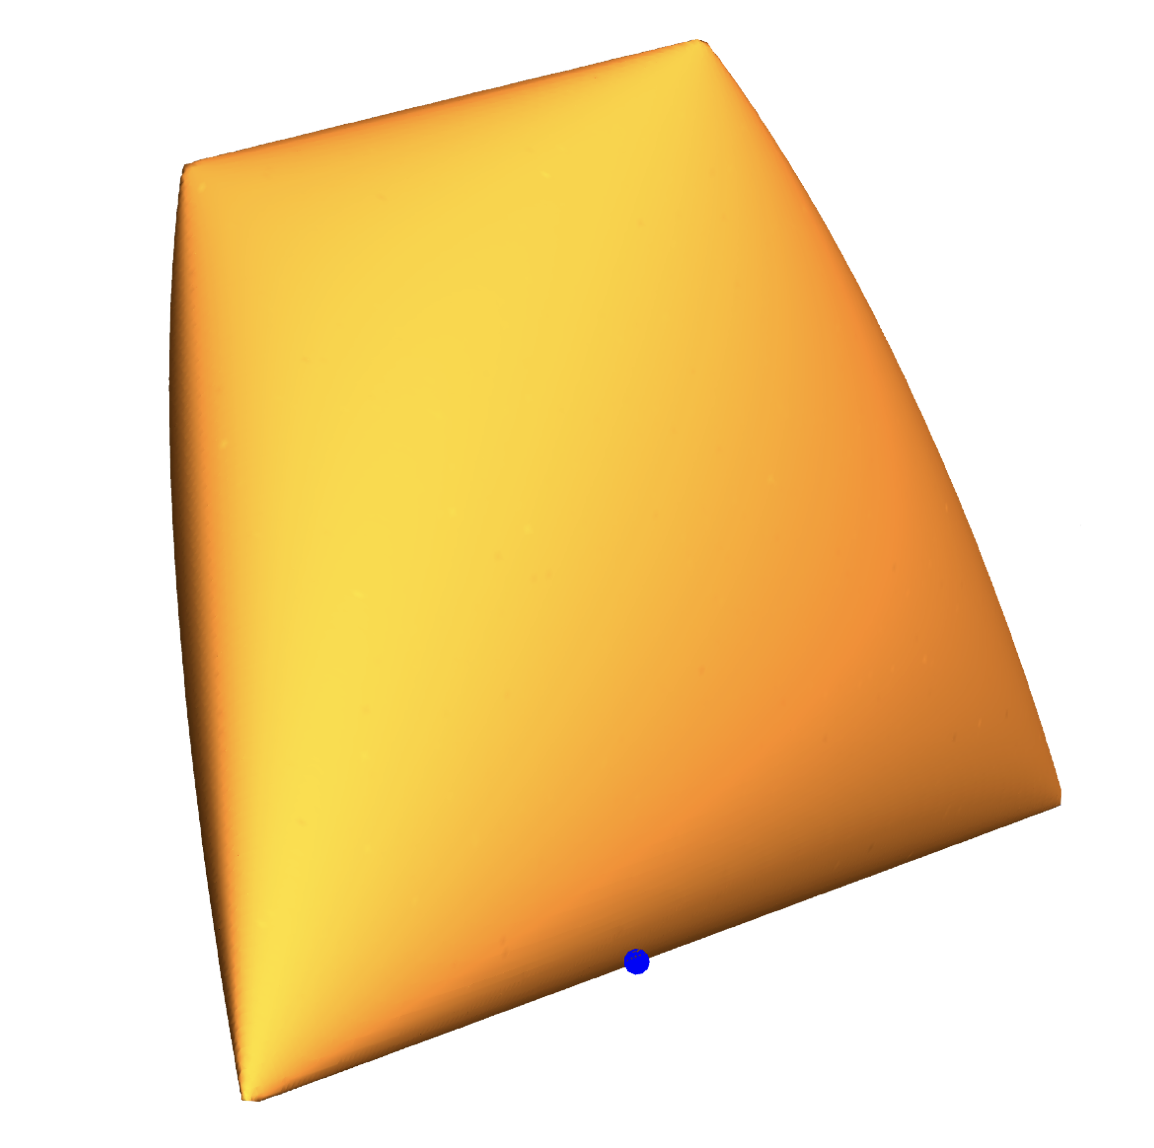
\includegraphics[width=0.5\linewidth]{images/spectrahedron-stride} 

}

\caption{An example spectrahedron.}\label{fig:SpectrahedronStride}
\end{figure}

Similarly, we say a matrix \(A \in \mathbb{S}^{n}\) is \textbf{positive definite} (PD) is its associated quadratic form is always positive, i.e.,
\[
x^\top A x > 0, \quad \forall x \in \mathbb{R}^{n}.
\]
We use \(\mathbb{S}^{n}_{++}\) to denote the set of \(n \times n\) PD matrices, and also write \(A \succ 0\) when the dimension is clear.

Below is set of equivalent characterizations of positive definite matrices.

\begin{lemma}[Positive Definite Matrices]
\protect\hypertarget{lem:PositiveDefinite}{}\label{lem:PositiveDefinite}

Let \(A \in \mathbb{S}^{n}\) be a symmetric matrix, the following statements are equivalent:

\begin{enumerate}
\def\labelenumi{\arabic{enumi}.}
\item
  A is positive definite.
\item
  \(x^\top A x > 0, \forall x \in \mathbb{R}^{n}\).
\item
  All eigenvalues of \(A\) are strictly positive.
\item
  All \(n\) leading principal minors of \(A\) are strictly positive.
\item
  The coefficients of \(p_A(\lambda)\) strictly alternate in sign, i.e., \((-1)^{n-k} p_k > 0\) for \(k=0,\dots,n-1\), where \(p_A(\lambda) = \det (A - \lambda \mathrm{I}_n)\) is the characteristics polynomial of \(A\).
\item
  There exists a factorization \(A = BB^\top\) with \(B\) square and nonsingular (full-rank).
\end{enumerate}

\end{lemma}

\textbf{Schur Complements}. A useful technique to check whether a matrix is positive (semi-)definite is to use the Schur Complements. Consider a block-partitioned matrix
\begin{equation}
M = \begin{bmatrix} A & B \\ B^\top& C \end{bmatrix},
\label{eq:block-mat-M}
\end{equation}
where \(A\) and \(C\) are symmetric matrices.
If \(A\) is invertible, then the Schur complement of \(A\) is
\[
M / A = C - B^\top A^{-1}B.
\]
Similarly, if \(C\) is invertible, then the Schur complement of \(C\) is
\[
M / C = A - B C^{-1}B^\top.
\]

We have the following result relating the Schur Complements to positive (semi-)definiteness.

\begin{proposition}[Schur Complements and PSD]
\protect\hypertarget{prp:SchurPSD}{}\label{prp:SchurPSD}

Consider the block-partitioned matrix \(M\) in \eqref{eq:block-mat-M},

\begin{itemize}
\item
  \(M\) is positive definite if and only if both \(A\) and \(M/A\) are positive definite:
  \[
  M \succ 0 \Leftrightarrow A \succ 0, M/A = C - B^\top A^{-1}B \succ 0.
  \]
\item
  \(M\) is positive definite if and only if both \(C\) and \(M/C\) are positive definite:
  \[
  M \succ 0 \Leftrightarrow C \succ 0, M/C = A - B C^{-1}B^\top\succ 0.
  \]
\item
  If \(A\) is positive definite, then \(M\) is positive semidefinite if and only if \(M/A\) is positive semidefinite:
  \[
  \text{If } A \succ 0, \text{ then } M \succeq 0 \Leftrightarrow M / A \succeq 0.
  \]
\item
  If \(C\) is positive definite, then \(M\) is positive semidefinite if and only if \(M/C\) is positive semidefinite:
  \[
  \text{If } C \succ 0, \text{ then } M \succeq 0 \Leftrightarrow M / C \succeq 0.
  \]
\end{itemize}

\end{proposition}

\hypertarget{geometric-properties}{%
\subsection{Geometric Properties}\label{geometric-properties}}

The set \(\mathbb{S}^{n}_{+}\) is a proper cone (cf.~Definition \ref{def:ProperCone}). Its interior is \(\mathbb{S}^{n}_{++}\). Under the inner product
\[
\langle A, B \rangle = \mathrm{tr}(AB^\top), \quad A,B \in \mathbb{R}^{n \times n},
\]
the PSD cone \(\mathbb{S}^{n}_{+}\) is self-dual.

Next we want to characterize the face of the PSD cone. We first present the following lemma which will turn out to be useful afterwards.

\begin{lemma}[Range of PSD Matrices]
\protect\hypertarget{lem:PSDRange}{}\label{lem:PSDRange}Let \(A,B \in \mathbb{S}^{n}_{+}\), then we have
\begin{equation}
\mathrm{Range}(A) \subseteq \mathrm{Range}(A + B),
\label{eq:Range-PSD}
\end{equation}
where \(\mathrm{Range}(A)\) denotes the span of the column vectors of \(A\).
\end{lemma}

\begin{proof}
For any symmetric matrix \(S\), we know
\[
\mathrm{Range}(S) = \mathrm{ker}(S)^{\perp}.
\]
Therefore, to prove \eqref{eq:Range-PSD}, it is equivalent to prove
\[
\mathrm{ker}(A) \supseteq \mathrm{ker}(A + B).
\]
Pick any \(u \in \mathrm{ker}(A + B)\), we have
\[
(A + B) u = 0 \Rightarrow u ^\top(A + B) u = 0 \Rightarrow u^\top A u + u^\top B u = 0 \Rightarrow u^\top A u = u^\top B u = 0,
\]
where the last derivation is due to \(A, B \succeq 0\). Now that we have \(u^\top A u = 0\), we claim that \(Au = 0\) must hold, i.e., \(u \in \mathrm{ker}(A)\). To see this, write
\[
u = \sum_{i=1}^n a_i v_i,
\]
where \(a_i = \langle u, v_i \rangle\) and \(v_i,i=1,\dots,n\) are the eigenvectors of \(A\) corresponding to eigenvalues \(\lambda_i,i=1,\dots,n\). Then we have
\[
Au = \sum_{i=1}^n a_i A v_i = \sum_{i=1}^n a_i \lambda_i v_i,
\]
and
\[
u^\top A u = \sum_{i=1}^n \lambda_i a_i^2 = 0.
\]
Since \(\lambda_i \geq 0, a_i^2 \geq 0\), we have
\[
\lambda_i a_i^2 = 0, \forall i = 1,\dots,n.
\]
This indicates that if \(\lambda_i > 0\), then \(a_i = 0\). Therefore, \(a_i\) can only be nonzero for \(\lambda_i = 0\), which leads to
\[
Au = \sum_{i=1}^n a_i \lambda_i v_i = 0.
\]
Therefore, \(u \in \mathrm{ker}(A)\), proving the result.
\end{proof}

Lemma \ref{lem:PSDRange} indicates that if \(A \succeq B\), then \(\mathrm{Range}(B) \subseteq \mathrm{Range}(A)\). What about the reverse?

\begin{lemma}[Extend Line Segment]
\protect\hypertarget{lem:Extension}{}\label{lem:Extension}Let \(A,B \in \mathbb{S}^{n}_{+}\), if \(\mathrm{Range}(B) \subseteq \mathrm{Range}(A)\), then there must exist \(C \in \mathbb{S}^{n}_{+}\) such that
\[
A \in (B,C),
\]
i.e., the line segment from \(B\) to \(A\) can be extended past \(A\) within \(\mathbb{S}^{n}_{+}\).
\end{lemma}

\begin{proof}
Since \(\mathrm{Range}(B) \subseteq \mathrm{Range}(A)\), we have
\[
\mathrm{ker}(A) \subseteq \mathrm{ker}(B).
\]
Now consider extending the line segment past \(A\) to
\[
C_{\alpha} = A + \alpha(A - B) = (1+\alpha) A - \alpha B,
\]
with some \(\alpha > 0\). We want to show that there exists \(\alpha > 0\) such that \(C_{\alpha} \succeq 0\).

Pick \(u \in \mathbb{R}^{n}\), then either \(u \in \mathrm{ker}(B)\) or \(u \not\in \mathrm{ker}(B)\). If \(u \in \mathrm{ker}(B)\), then
\[
u^\top C_{\alpha} u = (1+\alpha) u^\top A u - \alpha u^\top B u = (1+\alpha) u^\top A u \geq 0.
\]
If \(u \not\in \mathrm{ker}(B)\), then due to \(\mathrm{ker}(A) \subseteq \mathrm{ker}(B)\), we have \(u \not\in \mathrm{ker}(A)\) as well. As a result, we have
\begin{equation}
u^\top C_{\alpha} u = (1+\alpha) u^\top A u - \alpha u^\top B u = (1+\alpha) u^\top A u \lparen{ 1- \frac{\alpha}{1+\alpha} \frac{u^\top B u}{u^\top A u} }.
\label{eq:prove-extension-1}
\end{equation}
Since
\[
\max_{u: u \not\in \mathrm{ker}(A)} \frac{u^\top B u}{u^\top A u} \leq \frac{\lambda_{\max}(B)}{\lambda_{\min,>0}(A)},
\]
where \(\lambda_{\min,>0}(A)\) denotes the minimum positive eigenvalue of \(A\), we can always choose \(\alpha\) sufficiently small to make \eqref{eq:prove-extension-1} nonnegative. Therefore, there exists \(\alpha > 0\) such that \(C_{\alpha} \succeq 0\).
\end{proof}

In fact, from Lemma \ref{lem:PSDRange} we can induce a corollary.

\begin{corollary}[Range of PSD Matrices]
\protect\hypertarget{cor:PSDRange}{}\label{cor:PSDRange}Let \(A, B \in \mathbb{S}^{n}_{+}\), then we have
\[
\mathrm{Range}(A + B) = \mathrm{Range}(A) + \mathrm{Range}(B),
\]
with ``\(+\)'' the Minkowski sum.
\end{corollary}

\begin{exercise}
Let \(A,B \in \mathbb{S}^{n}_{+}\), show that \(\langle A, B \rangle = 0\) if and only if \(\mathrm{Range}(A) \perp \mathrm{Range}(B)\).
\end{exercise}

For a subset \(T \subseteq \mathbb{S}^{n}_{+}\), we use \(\mathrm{face}(T,\mathbb{S}^{n}_{+})\) to denote the smallest face of \(\mathbb{S}^{n}_{+}\) that contains \(T\). We first characterize the smallest face that contains a given PSD matrix, i.e., \(\mathrm{face}(A,\mathbb{S}^{n}_{+})\) for \(A\succeq 0\). Clearly, if \(A\) is PD, then \(\mathrm{face}(A, \mathbb{S}^{n}_{+}) = \mathbb{S}^{n}_{+}\) is the entire cone. If \(A\) is PSD but singular with rank \(r < n\), then \(A\) has the following spectral decomposition
\[
Q^\top A Q = \begin{bmatrix} \Lambda & 0 \\ 0 & 0 \end{bmatrix},
\]
where \(\Lambda \in \mathbb{S}^{r}_{++}\) is a diagonal matrix with the \(r\) nonzero eigenvalues of \(A\), and \(Q \in \mathrm{O}(n)\) is orthogonal. If
\[
A = \lambda B + (1-\lambda)C, \quad B,C \in \mathbb{S}^{n}_{+},\lambda \in (0,1),
\]
then multiplying both sides by \(Q^\top\) and \(Q\) we have
\[
\begin{bmatrix} \Lambda & 0 \\ 0 & 0 \end{bmatrix} = Q^\top A Q = \lambda Q^\top B Q + (1-\lambda) Q^\top C Q.
\]
Therefore, it must hold that
\[
Q^\top B Q = \begin{bmatrix} B_1 & 0 \\ 0 & 0 \end{bmatrix}, \quad Q^\top C Q = \begin{bmatrix} C_1 & 0 \\ 0 & 0 \end{bmatrix}, \quad B_1 \in \mathbb{S}^{r}_{+}, C_1 \in \mathbb{S}^{r}_{+},
\]
which is equivalent to
\[
B = Q \begin{bmatrix} B_1 & 0 \\ 0 & 0 \end{bmatrix} Q^\top, C = Q \begin{bmatrix} C_1 & 0 \\ 0 & 0 \end{bmatrix} Q^\top, \quad B_1 \in \mathbb{S}^{r}_{+}, C_1 \in \mathbb{S}^{r}_{+}.
\]
We conclude that \(\mathrm{face}(A,\mathbb{S}^{n}_{+})\) must contain the set
\begin{equation}
G:=  \left\{ Q \begin{bmatrix} X & 0 \\ 0 & 0 \end{bmatrix} Q^\top\ \middle\vert\ X \in \mathbb{S}^{r}_{+} \right\} .
\label{eq:face-of-A-psd}
\end{equation}

\begin{exercise}
Show that \(G\) in \eqref{eq:face-of-A-psd} is a face of \(\mathbb{S}^{n}_{+}\), i.e., (i) \(G\) is convex; (ii) \(u \in (x,y), u \in G, x,y \in \mathbb{S}^{n}_{+} \Rightarrow x,y \in G\).
\end{exercise}

As a result, we have \(\mathrm{face}(A,\mathbb{S}^{n}_{+}) = G\).

More general faces of the PSD cone \(\mathbb{S}^{n}_{+}\) can be characterized as follows (Theorem 3.7.1 in \citep{wolkowicz12book-sdp}).

\begin{theorem}[Faces of the PSD Cone]
\protect\hypertarget{thm:FacePSD}{}\label{thm:FacePSD}A set \(F \subseteq \mathbb{S}^{n}_{+}\) is a face if and only if there exists a subspace \(L \subseteq \mathbb{R}^{n}\) such that
\[
F = \{ X \in \mathbb{S}^{n}_{+} \mid \mathrm{Range}(X) \subseteq L \}.
\]
\end{theorem}

\begin{proof}
It is easy to prove the ``\textbf{If}'' direction using Lemma \ref{lem:PSDRange}.

First we show \(F\) is convex. Pick \(A,B \in F\). We have \(\mathrm{Range}(A) \subseteq L\) and \(\mathrm{Range}(B) \subseteq L\). Let \(v_1,\dots,v_m\) be a set of basis spanning \(L\). We have that, for any \(u \in \mathbb{R}^{n}\),
\begin{equation}
\begin{split}
A u \in L & \Rightarrow Au = \sum_{i=1}^m a_i v_i, \\
B u \in L & \Rightarrow Bu = \sum_{i=1}^m b_i v_i. 
\end{split}
\end{equation}
So for any \(\lambda \in [0,1]\), we have
\[
(\lambda A + (1-\lambda) B) u = \lambda Au + (1-\lambda) Bu = \sum_{i=1}^m (\lambda a_i + (1-\lambda) b_i ) v_i \in L,
\]
implying \(\lambda A + (1-\lambda) B \in F\) for any \(\lambda \in [0,1]\).

Now we show that:
\[
X \in (A,B), X \in F, A,B \in \mathbb{S}^{n}_{+} \Rightarrow A, B \in F.
\]
From \(X = \lambda A + (1-\lambda) B\) for some \(\lambda \in (0,1)\), and invoking Lemma \ref{lem:PSDRange}, we have
\begin{equation}
\begin{split}
\mathrm{Range}(X) & = \mathrm{Range}(\lambda A + (1-\lambda) B) \supseteq \mathrm{Range}(\lambda A) = \mathrm{Range}(A) \\
\mathrm{Range}(X) & = \mathrm{Range}(\lambda A + (1-\lambda) B) \supseteq \mathrm{Range}((1-\lambda) B) = \mathrm{Range}(B).
\end{split}
\end{equation}
Since \(\mathrm{Range}(X) \subseteq L\) due to \(X \in F\), we have
\[
\mathrm{Range}(A) \subseteq L, \quad \mathrm{Range}(B) \subseteq L,
\]
leading to \(A,B \in F\).

The proof for the ``\textbf{Only If}'' direction can be found in Theorem 3.7.1 of \citep{wolkowicz12book-sdp}.
\end{proof}

\hypertarget{semidefinite-programming}{%
\section{Semidefinite Programming}\label{semidefinite-programming}}

\hypertarget{spectrahedra}{%
\subsection{Spectrahedra}\label{spectrahedra}}

Recall the definition of a polyhedron in \eqref{eq:polyhedron}, i.e., a vector \(x\) constrained by finitely many linear inequalities. The feasible set of a Linear Program is a polyhedron.

Similarly, we define a \textbf{spectrahedron} as a set defined by finitely many \textbf{linear matrix inequalities} (LMIs). Spectrahedra are the feasible sets of Semidefinite Programs (SDPs).

A linear matrix inequality has the form
\[
A_0 + \sum_{i=1}^m A_i x_i \succeq 0,
\]
where \(A_i \in \mathbb{S}^{n},i=0,\dots,m\) are given symmetric matrices. Correspondingly, a spectrahedron is defined by finitely many LMIs.

\begin{definition}[Spectrahedron]
\protect\hypertarget{def:Spectrahedron}{}\label{def:Spectrahedron}A set \(S \subseteq \mathbb{R}^{m}\) is a spectrahedron if it has the form
\[
S =  \left\{ x \in \mathbb{R}^{m} \ \middle\vert\ A_0 + \sum_{i=1}^m x_i A_i \succeq 0 \right\} ,
\]
for given symmetric matrices \(A_0,A_1,\dots,A_m \in \mathbb{S}^{n}\).
\end{definition}

Note that there is no less of generality in defining a spectrahedron using a single LMI. For example, in the case of a set defined by two LMIs:
\[
S =  \left\{ x \in \mathbb{R}^{m} \ \middle\vert\ A_0 + \sum_{i=1}^m x_i A_i \succeq 0, B_0 + \sum_{i=1}^m x_i B_i \succeq 0  \right\} , A_i \in \mathbb{S}^{n}, B_i \in \mathbb{S}^{d},
\]
we can compress the two LMIs into a single LMI by putting \(A_i\) and \(B_i\) along the diagonal:
\[
S =  \left\{ x \in \mathbb{R}^{m} \ \middle\vert\ \begin{bmatrix} A_0 & \\ & B_0 \end{bmatrix} + \sum_{i=1}^m x_i \begin{bmatrix} A_i & \\ & B_i \end{bmatrix} \succeq 0  \right\} .
\]

Leveraging (5) of Lemma \ref{lem:PositiveSemidefinite}, we know that a PSD constraint is equivalent to weakly alternating signs of the characteristic polynomial of the given matrix. Therefore, a spectrahedron is defined by finitely many polynomial inequalities, i.e., a spectrahedron is a (convex) \textbf{basic semialgebraic set}, as seen in the following example \citep{blekherman12book-semidefinite}. Another example is provided in Fig. \ref{fig:SpectrahedronStride}.

\begin{example}[Elliptic Curve]
\protect\hypertarget{exm:EllipticCurve}{}\label{exm:EllipticCurve}

Consider the spectrahedron in \(\mathbb{R}^{2}\) defined by
\[
 \left\{ (x,y) \in \mathbb{R}^{2} \ \middle\vert\ A(x,y) = \begin{bmatrix} x+1 & 0 & y \\ 0 & 2 & -x-1 \\ y & -x-1 & 2 \end{bmatrix} \succeq 0  \right\} .
\]
To obtain scalar inequalities defining the set, let
\[
p_A(\lambda) = \det (\lambda I - A(x,y)) = \lambda^3 + p_2 \lambda^2 + p_1 \lambda + p_0
\]
be the characteristic polynomial of \(A(x,y)\). \(A(x,y) \succeq 0\) is then equivalent to the coefficients weakly alternating in sign:
\begin{equation}
\begin{split}
p_2 & = -(x+5) \leq 0, \\
p_1 & = -x^2 + 2x - y^2 + 7 \geq 0, \\
p_0 & = -(3+ x -x^3 -3x^2 - 2y^2) \leq 0.
\end{split}
\end{equation}
We can use the following Matlab script to plot the set shown in Fig. \ref{fig:EllipticCurve}. (The code is also available at \href{https://github.com/ComputationalRobotics/Semidefinite-Examples}{here}.) As we can see, the spectrahedron is convex, but it is not a polyhedron.

\begin{Shaded}
\begin{Highlighting}[]
\VariableTok{x} \OperatorTok{=} \OperatorTok{{-}}\FloatTok{2}\OperatorTok{:}\FloatTok{0.01}\OperatorTok{:}\FloatTok{2}\OperatorTok{;} 
\VariableTok{y} \OperatorTok{=} \OperatorTok{{-}}\FloatTok{2}\OperatorTok{:}\FloatTok{0.01}\OperatorTok{:}\FloatTok{2}\OperatorTok{;} 
\NormalTok{[}\VariableTok{X}\OperatorTok{,}\VariableTok{Y}\NormalTok{] }\OperatorTok{=} \VariableTok{meshgrid}\NormalTok{(}\VariableTok{x}\OperatorTok{,}\VariableTok{y}\NormalTok{)}\OperatorTok{;}

\VariableTok{ineq} \OperatorTok{=}\NormalTok{ (}\OperatorTok{{-}}\VariableTok{X} \OperatorTok{{-}} \FloatTok{5} \OperatorTok{\textless{}=} \FloatTok{0}\NormalTok{) }\OperatorTok{\&} \OperatorTok{...}
\NormalTok{    (}\OperatorTok{{-}}\VariableTok{X}\OperatorTok{.\^{}}\FloatTok{2} \OperatorTok{+} \FloatTok{2}\OperatorTok{*}\VariableTok{X} \OperatorTok{{-}} \VariableTok{Y}\OperatorTok{.\^{}}\FloatTok{2} \OperatorTok{+} \FloatTok{7} \OperatorTok{\textgreater{}=}\FloatTok{0}\NormalTok{) }\OperatorTok{\&} \OperatorTok{...}
\NormalTok{    (}\FloatTok{3} \OperatorTok{+} \VariableTok{X} \OperatorTok{{-}} \VariableTok{X}\OperatorTok{.\^{}}\FloatTok{3} \OperatorTok{{-}} \FloatTok{3}\OperatorTok{*}\VariableTok{X}\OperatorTok{.\^{}}\FloatTok{2} \OperatorTok{{-}} \FloatTok{2}\OperatorTok{*}\VariableTok{Y}\OperatorTok{.\^{}}\FloatTok{2} \OperatorTok{\textgreater{}=} \FloatTok{0}\NormalTok{)}\OperatorTok{;}

\VariableTok{h} \OperatorTok{=} \VariableTok{pcolor}\NormalTok{(}\VariableTok{X}\OperatorTok{,}\VariableTok{Y}\OperatorTok{,}\VariableTok{double}\NormalTok{(}\VariableTok{ineq}\NormalTok{)) }\OperatorTok{;}
\VariableTok{h}\NormalTok{.}\VariableTok{EdgeColor} \OperatorTok{=} \SpecialStringTok{\textquotesingle{}none\textquotesingle{}} \OperatorTok{;}
\end{Highlighting}
\end{Shaded}

\begin{figure}

{\centering 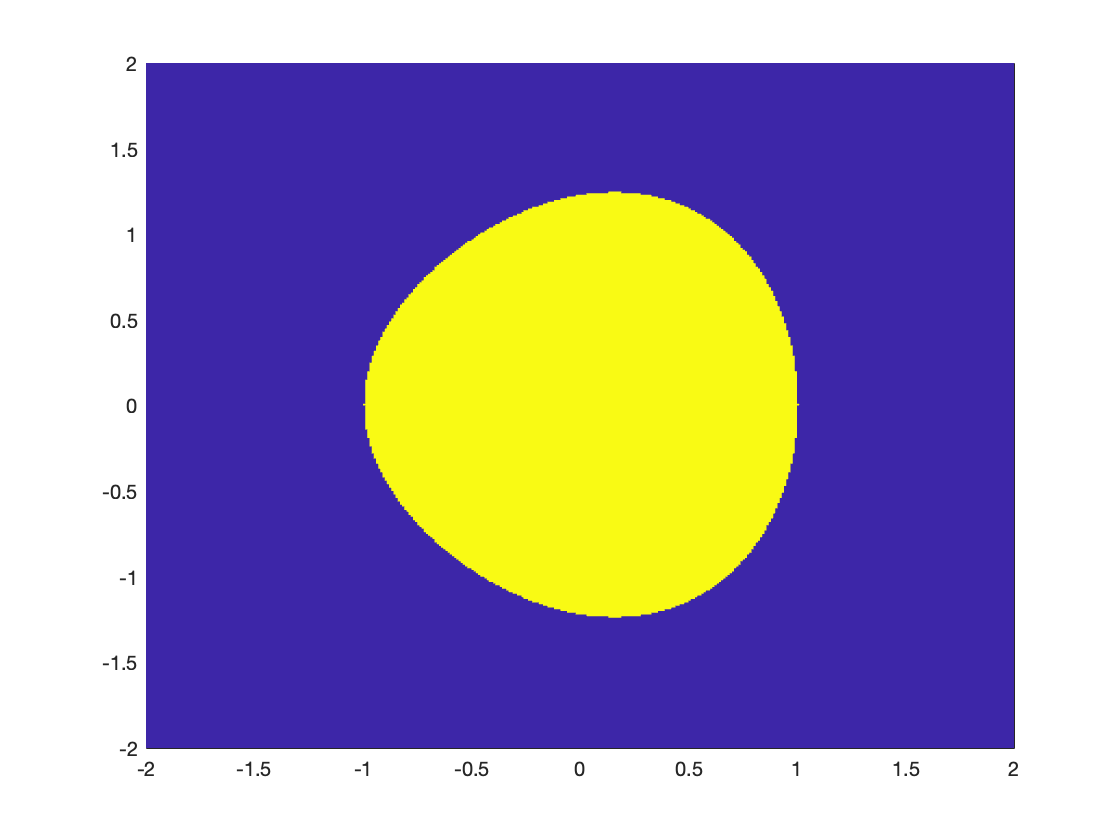
\includegraphics[width=0.6\linewidth]{images/elliptic_curve} 

}

\caption{Elliptic Curve.}\label{fig:EllipticCurve}
\end{figure}

\end{example}

\hypertarget{formulation-and-duality}{%
\subsection{Formulation and Duality}\label{formulation-and-duality}}

Semidefinite programs (SDPs) are linear optimization problems over spectrahedra. A standard SDP in \textbf{primal} form is written as
\begin{equation}
\boxed{
\begin{split}
p^\star = \min_{X \in \mathbb{S}^{n}} & \quad \langle C, X \rangle \\
\mathrm{s.t.}& \quad \mathcal{A}(X) = b, \\
& \quad X \succeq 0
\end{split}
}
\label{eq:SDP-P}
\end{equation}
where \(C \in \mathbb{S}^{n}\), \(b \in \mathbb{R}^{m}\), and the linear map \(\mathcal{A}: \mathbb{S}^{n} \rightarrow \mathbb{R}^{m}\) is defined as
\[
\mathcal{A}(X) := \begin{bmatrix} \langle A_1, X \rangle \\
\vdots \\ \langle A_i, X \rangle \\ \langle A_m, X \rangle \end{bmatrix}.
\]
Recall that \(\langle C, X \rangle = \mathrm{tr}(CX)\). The feasible set of \eqref{eq:SDP-P} is the intersection of the PSD cone (\(\mathbb{S}^{n}_{+}\)) and the affine subspace defined by \(\mathcal{A}(X) = b\).

Closely related to the primal SDP \eqref{eq:SDP-P} is the \textbf{dual} problem
\begin{equation}
\boxed{
\begin{split}
d^\star = \max_{y \in \mathbb{R}^{m}} & \quad \langle b, y \rangle \\
\mathrm{s.t.}& \quad C - \mathcal{A}^* (y) \succeq 0
\end{split}
}
\label{eq:SDP-D}
\end{equation}
where \(\mathcal{A}^{*}: \mathbb{R}^{m} \rightarrow \mathbb{S}^{n}\) is the \textbf{adjoint} map defined as
\[
\mathcal{A}^*(y) := \sum_{i=1}^m y_i A_i.
\]
Observe how the primal-dual SDP pair \eqref{eq:SDP-P}-\eqref{eq:SDP-D} parallels the primal-dual LP pair \eqref{eq:primal-lp}-\eqref{eq:dual-lp}.

\textbf{Weak duality}. We have a similar weak duality between the primal and dual. Pick any \(X\) that is feasible for the primal \eqref{eq:SDP-P} and \(y\) that is feasible for the dual \eqref{eq:SDP-D}, we have
\[
\boxed{\langle C, X \rangle - \langle b, y \rangle = \langle C, X \rangle - \langle \mathcal{A}(X), y \rangle = \langle C - \mathcal{A}^* (y), X \rangle \geq 0,}
\]
where the last inequality holds because both \(C - \mathcal{A}^*(y)\) and \(X\) are positive semidefinite. As a result, we have the weak duality
\[
d^\star \leq p^\star.
\]

Similar to the LP case, we will denote \(p^\star = +\infty\) if the primal is infeasible, \(p^\star = - \infty\) if the primal is unbounded below. We will denote \(d^\star = +\infty\) if the dual is unbounded above, and \(d^\star = -\infty\) if the dual is infeasible. We say the primal (or the dual) is \textbf{solvable} if it admits optimizers. We denote \(p^\star - d^\star\) as the \textbf{duality gap}.

Recall Theorem \ref{thm:LPStrongDuality} states that in LP, if at least one of the primal and dual is feasible, then strong duality holds (i.e., \(p^\star = d^\star = \{\pm \infty, \text{finite} \}\)). Unfortunately, this does not carry over to SDPs. Let us provide several examples.

\begin{example}[Failure of SDP Strong Duality]
\protect\hypertarget{exm:FailureSDPDuality}{}\label{exm:FailureSDPDuality}The first example, from \citep{ramana97mp-exact}, shows that even if both primal and dual are feasible, there could exist a nonzero duality gap. Consider the following SDP pair for some \(\alpha \geq 0\)
\[
\begin{cases}
\min_{X \in \mathbb{S}^{3}} & \alpha X_{11} \\
\mathrm{s.t.}& X_{22} = 0 \\
& X_{11} + 2 X_{23} = 1 \\
& \begin{bmatrix} X_{11} & X_{12} & X_{13} \\
* & X_{22} & X_{23} \\
* & * & X_{33} \end{bmatrix} \succeq 0 
\end{cases}, 
\begin{cases}
\max_{y \in \mathbb{R}^{2}} & y_2 \\
\mathrm{s.t.}& \begin{bmatrix} \alpha & 0 & 0 \\ 0 & 0 & 0 \\ 0 & 0 & 0 \end{bmatrix} \succeq \begin{bmatrix} y_2 & 0 & 0 \\ 0 & y_1 & y_2 \\ 0 & y_2 & 0 \end{bmatrix}
\end{cases}
\]
To examine the primal feasible set, let us pick the bottom-right \(2\times 2\) submatrix of \(X\). The determinant of this submatrix needs to be nonnegative (due to (4) of Lemma \ref{lem:PositiveSemidefinite}):
\[
X_{22} X_{33} - X_{23}^2 \geq 0.
\]
Because \(X_{22} = 0\), we have \(X_{23} = 0\) and hence \(X_{11} = 1\). Therefore, \(p^\star = \alpha\) is attained.

To examine the dual feasible set, pick the bottom-right \(2 \times 2\) submatrix of
\[
\begin{bmatrix} \alpha - y_2 & 0 & 0 \\ 0 & - y_1 & -y_2 \\ 0 & -y_2 & 0 \end{bmatrix} \succeq 0,
\]
we have \(y_2 = 0\). As a result, \(d^\star = 0\), and strong duality fails.

The second example, from \citep{todd01an-semidefinite}, shows that the duality gap can even be infinite. Consider the primal-dual SDP
\[
\begin{cases}
\min_{X \in \mathbb{S}^{2}} & 0 \\
\mathrm{s.t.}& X_{11} = 0 \\
& X_{12} = 1 \\
& \begin{bmatrix} X_{11} & X_{12} \\ * & X_{22} \end{bmatrix} \succeq 0
\end{cases},
\begin{cases}
\max_{y \in \mathbb{R}^{2}} & 2 y_2 \\
\mathrm{s.t.}& \begin{bmatrix} - y_1 & - y_2 \\ - y_2 & 0 \end{bmatrix} \succeq 0 
\end{cases}
\]
Clearly, the primal is infeasible because
\[
\begin{bmatrix} 0 & 1 \\ 1 & X_{22} \end{bmatrix}
\]
can never be PSD. So \(p^\star = + \infty\). The dual problem, however, is feasible. From the PSD constraint we have \(y_2 = 0\) and \(d^\star = 0\). Therefore, the duality gap is infinite.

The third example, from \citep{todd01an-semidefinite}, shows that even when the duality gap is zero, the primal or dual problem may not admit optimizers. Consider the primal-dual SDP
\[
\begin{cases}
\min_{X \in \mathbb{S}^{2}} & 2 X_{12} \\
\mathrm{s.t.}& - X_{11} = -1 \\
& - X_{22} = 0 \\
& \begin{bmatrix} X_{11} & X_{12} \\ * & X_{22} \end{bmatrix} \succeq 0 
\end{cases},
\begin{cases}
\max_{y \in \mathbb{R}^{2}} & - y_1 \\
\mathrm{s.t.}& \begin{bmatrix} y_1 & 1 \\ 1 & y_2 \end{bmatrix} \succeq 0
\end{cases}
\]
To examine the primal feasible set, we have
\[
\begin{bmatrix} 1 & X_{12} \\ X_{12} & 0 \end{bmatrix} \succeq 0
\]
implies \(X_{12} = 0\). Hence the primal feasible set only has one point and \(p^\star = 0\). The dual feasible set reads
\[
y_1 y_2 \geq 1,\quad  y_1 \geq 0, \quad y_2 \geq 0,
\]
and we want to minimize \(y_1\). Clearly, \(d^\star = 0\) but it is not attainable. Therefore, strong duality holds but the dual problem is not solvable.
\end{example}

The examples above are somewhat ``pathological'' and they show that SDPs in general can be more complicated that LPs. It turns out, with the addition of \textbf{Slater's condition}, i.e., \textbf{strict feasibility} of the primal and dual, we can recover nice results parallel to those of LP.

\begin{theorem}[SDP Strong Duality]
\protect\hypertarget{thm:SDPStrongDuality}{}\label{thm:SDPStrongDuality}Assume both the primal SDP \eqref{eq:SDP-P} and the dual SDP \eqref{eq:SDP-D} are \emph{strictly feasible}, i.e., there exists \(X \succ 0\) such that \(\mathcal{A}(X)=b\) for the primal and there exists \(y \in \mathbb{R}^{m}\) such that \(C - \mathcal{A}^* (y) \succ 0\) for the dual, then strong duality holds, i.e., both problems are solvable and admit optimizers, and \(p^\star = d^\star\) equals to some finite number.

Further, a pair of primal-dual feasible points \((X,y)\) is optimal if and only if
\[
\langle C, X \rangle = \langle b, y \rangle \Leftrightarrow \langle C - \mathcal{A}^* (y), X \rangle = 0 \Leftrightarrow (C - \mathcal{A}^* (y)) X = 0.
\]
\end{theorem}

One can relax the requirement of both primal and dual being strictly feasible to only one of them being strictly feasible, and similar results would hold. Precisely, if the primal is bounded below and strictly feasible, then \(p^\star = d^\star\) and the dual is solvable. If the dual is bounded above and strictly feasible, then \(p^\star = d^\star\) and the primal is solvable \citep{nie23book-moment}.

\begin{example}[SDP Strong Duality]
\protect\hypertarget{exm:SuccessSDPDuality}{}\label{exm:SuccessSDPDuality}Consider the following primal-dual SDP pair
\[
\begin{cases}
\min_{X \in \mathbb{S}^{2}} & 2 X_{11} + 2 X_{12} \\
\mathrm{s.t.}& X_{11} + X_{22} = 1 \\
& \begin{bmatrix} X_{11} & X_{12} \\ * & X_{22} \end{bmatrix} \succeq 0 
\end{cases},
\begin{cases}
\max_{y \in \mathbb{R}^{}} & y \\
\mathrm{s.t.}& \begin{bmatrix} 2 - y & 1 \\ 1 & - y \end{bmatrix} \succeq 0
\end{cases}
\]
Choose
\[
X = \begin{bmatrix} 0.5 & 0 \\ 0 & 0.5 \end{bmatrix} \succ 0
\]
we see the primal is strictly feasible.
Choose \(y = -1\), we have
\[
\begin{bmatrix} 3 & 1 \\ 1 & 1 \end{bmatrix} \succ 0
\]
and the dual is strictly feasible. Therefore, strong duality holds.

In this case, pick the pair of primal-dual feasible points
\[
X^\star = \begin{bmatrix} \frac{2 - \sqrt{2}}{4} & - \frac{1}{2 \sqrt{2}} \\ - \frac{1}{2 \sqrt{2}} & \frac{2 + \sqrt{2}}{4} \end{bmatrix}, \quad y^\star = 1 - \sqrt{2},
\]
we have
\[
\langle C, X^\star \rangle = 1-\sqrt{2} = \langle b, y^\star \rangle,
\]
and both \(X^\star\) and \(y^\star\) are optimal.
\end{example}

\hypertarget{geometric-properties-1}{%
\subsection{Geometric Properties}\label{geometric-properties-1}}

\hypertarget{interior-point-algorithm}{%
\section{Interior Point Algorithm}\label{interior-point-algorithm}}

  \bibliography{book.bib}

\end{document}
